\documentclass[]{article}
\setcounter{secnumdepth}{0}
\usepackage[utf8]{inputenc}
\usepackage{authblk}
\usepackage{setspace}
\usepackage[margin=1.25in]{geometry}
\usepackage{graphicx}
\graphicspath{ {./figures/} }
\usepackage{subcaption}
\usepackage{amsmath}
\usepackage{lineno}
\usepackage[export]{adjustbox}
\usepackage{float}
\usepackage[labelfont=bf,justification=raggedright,singlelinecheck=false]{caption}
\usepackage{fancyhdr}
\let\href\undefined
\usepackage[hidelinks]{hyperref}
\usepackage[capitalize]{cleveref}
\usepackage{xspace}
\usepackage{xcolor}
\usepackage{multirow}
\linenumbers

%%%%%% Running header %%%%%%
\pagestyle{fancy}
\fancyhead[R]{\textbf{machine learning local adaptation}}

%%%%%% Commands %%%%%%
\newcommand{\dfir}{Douglas fir}
\newcommand{\ecolocator}{\texttt{EcoLocator}\xspace}

\newcommand{\beginsupplement}{%
    \setcounter{table}{0}
    \renewcommand{\thetable}{S\arabic{table}}%
    \setcounter{figure}{0}
    \renewcommand{\thefigure}{S\arabic{figure}}%
    \renewcommand{\theHtable}{supp.\arabic{table}}%
    \renewcommand{\theHfigure}{supp.\arabic{figure}}%
}

\newcommand{\sbt}[1]{\textcolor{red}{\textbf{SBT: #1}}}


%%%%%% Bibliography %%%%%%
\usepackage[style=authoryear,
citestyle=authoryear,
sorting=nyt,
natbib=true]{biblatex}
\addbibresource{ELrefs.bib}

%%%%%% Title %%%%%%
\title{Supervised machine learning jointly predicts geographic location
and climate of origin from genotypes}

%%%%%% Authors %%%%%%
\author[1*]{Jordan Rodriguez}
\author[2]{Richard Cronn}
\author[1]{Silas Tittes}
\author[1]{Andrew D. Kern}

%%%%%% Affiliations %%%%%%
\affil[1]{Department of Biology, University of Oregon, Eugene, USA.}
\affil[2]{Pacific Northwest Research Station, USDA Forest Service, Corvallis, Oregon, USA.}
\affil[*]{Address correspondence to: jrodrig8@uoregon.edu}

%%%%%% Spacing %%%%%%
\onehalfspacing

\begin{document}

\maketitle

%%%%%% Abstract %%%%%%
\begin{abstract}


\end{abstract}

%%%%%% Main Text %%%%%%

\section{Introduction}

Population genetic theory predicts that the distribution
of genetic variation within and between populations
is shaped by demographic history, spatial structure,
and selective pressures,
and thus carries information about the processes
that generate and maintain it
\citep{lewontin_genetic_1974, hartl_principles_1980, ellegren_determinants_2016}.
In spatially structured, locally adapted populations,
this variation encodes information about both geographic location
and climate of origin.
Geographic structure arises because local mating and limited dispersal
generate isolation by distance,
causing alleles to be more similar among neighboring individuals
than among those farther apart
\citep{wright_isolation_1943, slatkin_isolation_1993}.
Environmental selection, in contrast,
produces allele frequency clines that parallel ecological gradients,
as individuals carrying locally beneficial variants
enjoy higher fitness in particular environments
\citep{endler1977geographic, clausen_experimental_1948, kawecki_conceptual_2004}.
These two signals are partly separable:
neutral structure aligns primarily with geographic distance,
whereas adaptive signals track specific environmental
variables---temperature, moisture, seasonality
\citep{rellstab_practical_2015, hoban_finding_2016, tigano_genomics_2016, coop_using_2010}.
Yet the distinction is not clean,
because neutral demographic processes---historical
range expansions, bottlenecks, and genetic drift---can
themselves generate allele frequency gradients that mimic adaptive clines
\citep{excoffier_genetic_2009, novembre_spatial_2009}.

Local adaptation---the covariation of allele frequencies
with environmental gradients---emerges when spatially heterogeneous
selection outweighs the homogenizing effects of gene flow
\citep{savolainen_ecological_2013, lenormand_gene_2002}.
Beyond increasing local fitness,
it sustains genetic diversity across heterogeneous landscapes
by maintaining multiple adaptive alleles,
helping populations retain the variation
on which selection can act as environments change \citep{hereford_quantitative_2009}.
Classic models---Wright's isolation-by-distance
and stepping-stone frameworks \citep{wright_isolation_1943},
Levene's multiple-niche equilibrium \citep{levene_genetic_1953},
and Endler's cline theory \citep{endler1977geographic}---describe
how selection, migration, and drift interact
to shape predictable spatial patterns of variation.
More recent syntheses show that even modest selection
can create steep genomic clines under limited dispersal
\citep{tigano_genomics_2016, yeaman_genetic_2011},
whereas strong gene flow can swamp adaptive alleles
unless they are tightly linked or of large effect
\citep{slatkin_gene_1975}.

Understanding this relationship is especially urgent
as anthropogenic climate change rapidly disrupts the match
between populations and their environments \citep{lee_ipcc_2023}.
As suitable geographic ranges shift,
conservation managers face increasing pressure to anticipate
where populations will persist under novel conditions.
Classical approaches---common-garden experiments,
reciprocal transplant trials, and provenance tests---have
been indispensable in characterizing local adaptation,
but they are slow, costly,
and often limited in taxonomic or geographic scope
\citep{aitken_assisted_2013}.
Genomic tools offer a faster, more scalable alternative,
and the emerging field of landscape genomics
seeks to link spatial and environmental variation
with patterns of genetic diversity
\citep{manel_landscape_2003, rellstab_practical_2015}.
For forest species in particular,
genomic approaches are increasingly informing
seed transfer and assisted gene flow decisions
\citep{aitken_bemmels_2016}.

Genotype--environment association (GEA) methods
have become central to this effort.
These approaches identify putatively adaptive loci
by testing for statistical associations
between allele frequencies and environmental variables
\citep{rellstab_practical_2015}.
Univariate methods such as Bayenv2
\citep{guenther_bayenv2_2013},
latent factor mixed models
\citep{frichot_lfmm_2013},
and BayPass \citep{gautier_baypass_2015}
test loci one at a time against environmental predictors,
typically while controlling for population structure
through covariance matrices or latent factors.
These methods have been widely applied,
but they are limited in their ability to capture
polygenic adaptation involving many loci of small effect,
and they can be confounded by neutral demographic processes
that generate allele frequency gradients
correlated with environmental variation
\citep{lotterhos_whitlock_2015}.
Multivariate approaches address some of these limitations
by analyzing many loci and environmental predictors simultaneously.
Redundancy analysis (RDA) has proven effective
at detecting multilocus adaptive signatures
\citep{forester_comparing_2018, capblancq_rda_2021},
and gradient forest methods model
nonlinear allele--environment relationships
across the genome \citep{fitzpatrick_gradient_2015}.
More recently, the Weighted-Z Analysis (WZA) introduced
a window-based framework for aggregating
single-locus GEA statistics
into region-level summaries of adaptive signal
\citep{booker_wza_2024}.
Despite this progress,
most GEA methods share key limitations:
they are designed to \emph{test} for associations
between genotype and environment,
treating spatial population structure as a confounder
to be corrected for rather than a signal
to be modeled jointly with environment.
Consequently, they do not return an individual's
geographic coordinates, and---with the partial exception
of gradient-forest and genomic-offset approaches,
which project allele turnover under new climates
\citep{fitzpatrick_gradient_2015}---they do not
directly predict an individual's environment of origin
from its genotype.

We propose that machine learning (ML) can better leverage
information in the data to outperform the existing GEA methods,
while also providing a unique framing on the problem to gain new insights
and interpretations about geographic structure and climate of origin.
ML methods excel at extracting patterns
from high-dimensional data,
naturally handling nonlinear interactions among loci
and correlated environmental predictors
\citep{schrider_supervised_2018}.
\citet{battey_predicting_2020} demonstrated
that deep neural networks can predict
the geographic origin of an individual from its genotype alone,
using a tool called Locator.
By learning from multilocus patterns of isolation by distance,
Locator achieves high spatial accuracy,
but it does not incorporate environmental covariates
and therefore cannot distinguish adaptive signals
from neutral spatial structure.
Other recent work incorporates ecological context
more explicitly:
gradient forest methods link genomic variation
to environmental predictors to forecast
climate-driven maladaptation \citep{fitzpatrick_experimental_2021}, %ADK -- I replaced these citations. Not sure if these are right. Double check!
while multi-environment deep learning architectures
in agricultural genomics integrate weather, soil,
and other covariates to improve genotype performance prediction
across climates
\citep{washburn_predicting_2021, montesinoslopez_review_2021}.
What remains missing is an approach that jointly models
geographic and environmental prediction from genotypes,
capturing both neutral spatial structure
and adaptive environmental associations in a single framework.

Here we introduce \ecolocator,
a deep neural network that extends the geographic prediction
framework of \texttt{Locator} \citep{battey_predicting_2020} by jointly predicting
geographic location and climate of origin from genomic data.
Trained on georeferenced genotypes paired
with historical climate data,
the model learns multilocus associations
between genetic variation and environmental gradients.
When allele frequencies covary with climate variables,
the model can infer climate of origin directly from genotype.
By coupling spatial and environmental inference,
\ecolocator can leverage signals of both isolation by distance
and local adaptation.
We incorporate a downstream feature attribution method (SHAP \citep{lundberg_shap_2017})
to reveal how each input feature contributed to a given prediction,
identifying which variants contribute most strongly
to adaptive differentiation across landscapes.

We evaluate \ecolocator across a range of simulation parameterizations
to identify the conditions under which it performs best,
then apply it to an empirical dataset of coastal Douglas-fir
(\textit{Pseudotsuga menziesii} var.\ \textit{menziesii}).
Simulations provide a controlled setting
where evolutionary and environmental parameters are known,
allowing us to benchmark prediction accuracy against ground truth
before moving to more complex natural systems.

Coastal Douglas-fir is a member of the pine family
with a lineage dating to the Paleocene \citep{hermann_genus_1985}
and a natural range spanning extensive climatic
gradients along the North American Pacific coast from California
to British Columbia. Although most populations are characterized by
low genetic differentiation, high gene flow, and high outcrossing rates \citep{slavov_pollen_2005},
they still exhibit strong signatures of local adaptation,
with adaptive quantitative phenotypes tracking climatic features
such as winter cold temperatures and summer aridity \citep{stclair_genecology_2005}.
This combination of strong local adaptation and a long history
of ecological and silvicultural study
makes Douglas-fir a natural bridge
between controlled simulations and real-world management applications.
For the U.S. Forest Service,
seed source--climate relationships
are central to (mal)adaptation \citep{stclair_1912_2020},
reforestation success, and assisted migration planning \citep{stclair_genetic_2007}.
By matching genotypes to suitable environments,
\ecolocator complements long-standing knowledge on seed sourcing
(such as `seed zones' \citep{randall_forest_1996})
and expands the management options essential for sustaining
forest productivity and resilience under climate change.
Importantly, \ecolocator is not limited to this system;
it offers a pathway to inform management
in any species or taxon where
empirical knowledge of local adaptation is scarce.

By integrating population genetic theory,
simulation benchmarking, and empirical application,
our study presents the first open-source approach
for simultaneously inferring the geographic origin of a genotype
and the climate to which it is adapted---precisely
the information needed as shifting climates
outpace traditional experimental approaches.
These advances at the intersection of evolutionary biology
and computational science open new avenues
for understanding the genetic basis of adaptation,
with broad implications for conservation and species management.

\section{\ecolocator}

\sbt{We will probably be asked to stick to standard section style, but maybe put this as a subsection of the results?}

\ecolocator is an open-source Python package
for predicting the geographic origin and climate of origin
of individual genotypes, accessible via both a command-line 
interface and a programmatic Python API.
\footnote{Source code, installation instructions, and vignettes are available at \url{https://github.com/kr-colab/ecolocator} and \url{VIGNETTE URL}.}
\ecolocator does not depend on fixed assumptions about allele--environment relationships,
but learns directly from high-dimensional genomic
and environmental data (Figure~\ref{fig:1}).
By jointly predicting location and environmental variables,
it captures both spatial genetic structure
and signals of local adaptation,
providing a scalable, biologically informed approach
for studying complex evolutionary patterns.
Both the CLI and Python API accept standard genotype formats 
(VCF, Zarr, tab-delimited matrices), facilitating integration into existing 
genomic workflows whether scripting interactively or from the command line.

\subsection{Preprocessing}

\ecolocator converts genomic data from VCF, Zarr,
and tab-delimited matrix formats
into vectors of minor allele counts per individual
using the scikit-allel \citep{scikit_allel_v1.3.8} and NumPy \citep{numpy_v2.0.0} libraries.
Missing genotypes are imputed by drawing alleles
from a binomial distribution parameterized
by the site's allele frequency,
an approximation that preserves expected variation
while minimizing bias.
Sites can be filtered by a minor allele count threshold
to reduce noise from rare variants
that contribute little predictive signal.
Geographic coordinates are normalized to zero mean and unit variance,
and environmental covariates are standardized similarly
prior to training.

\subsection{Model architecture}

\ecolocator employs a multilayer perceptron with a shared trunk 
and two task-specific output heads, trained under a supervised 
learning framework on labeled datasets of genotypes paired with 
known geographic coordinates and climate variables. Input genotypes 
pass through a batch normalization layer before entering the shared 
trunk, which consists of dense layers with ELU activations and a 
central dropout layer for regularization. The trunk branches into 
two heads — one predicting 2D geographic coordinates (i.e., latitude and longitude), one predicting 
environmental covariates — each implemented as a small two-layer subnetwork. 
The network is optimized using the Adam optimizer with a custom multitask 
loss function (Equation 1), combining mean Euclidean distance for geographic 
prediction and MSE for environmental covariates, each scaled by an 
independently specified weight.

\begin{equation} \label{eq:1}
    \mathcal{L} = w_{\text{loc}} \left( \frac{1}{n} \sum_{i=1}^{n}
    \sqrt{(\hat{x}_i - x_i)^2 + (\hat{y}_i - y_i)^2} \right)
    + \, w_{\text{env}} \left( \frac{1}{np} \sum_{i=1}^{n} \sum_{j=1}^{p}
    (\hat{z}_{ij} - z_{ij})^2 \right)
\end{equation}
where $n$ is the number of training samples, $p$ is the number of environmental
covariates, $x_i$ and $y_i$ are the true longitude and latitude of sample $i$,
$\hat{x}_i$ and $\hat{y}_i$ are the predicted coordinates, $z_{ij}$ is the true
value of covariate $j$ for sample $i$, $\hat{z}_{ij}$ is the predicted value,
and $w_{\text{loc}}, w_{\text{env}} \geq 0$ are loss
weights (both defaulting to 1.0, see \Cref{fig:S1}).
The network is trained using a standard validation scheme in which a user-specified 
fraction of samples (default 0.9) is used for model fitting, while the remaining fraction is 
held out for validation, enabling convergence monitoring, early stopping, 
and adaptive learning rate reduction to prevent overfitting. 
By explicitly coupling geographic and climatic inference, the model captures 
both neutral spatial structure and environment-driven selection.



\begin{figure}[H]
    \adjustimage{width=1.1\textwidth,center}{figures/EcoLocatorARC.pdf}
    \caption{\ecolocator architecture. \textbf{Panel A} shows the training regime,
    with the inputs traversing the network in a supervised fashion; network weights 
    are updated through backpropagation until predictions are optimized towards the
    true value, with the process shown here in blue. Once trained, \ecolocator enters the prediction
    step, shown here in \textbf{Panel B}. Given genotypes alone, the trained network
    jointly predicts climate-of-origin and geographic location, shown in yellow. }
    \label{fig:1}
\end{figure}

In practice, an end-to-end \ecolocator analysis consists of five steps:
\begin{enumerate}
\item Assemble a training dataset consisting of genotype data 
in a supported format (VCF, Zarr, or tab-delimited matrix) 
and a sample metadata file pairing each individual with its 
known geographic coordinates and environmental covariate values. 
Samples to be predicted should have their coordinates and covariates 
left blank.

\item Train the model using \texttt{ecolocator train} (or the Python API), 
specifying the genotype file, sample metadata, and an output directory. 
The model is fit to jointly predict geographic origin and environmental 
covariates, with early stopping and adaptive learning rate reduction applied 
automatically.

\item Evaluate model performance using \texttt{ecolocator loo}, 
which iteratively holds out each sample with known coordinates, trains 
on the remainder, and predicts the held-out individual (leave-one-out cross validation). The resulting 
predictions can be compared against true values to assess spatial and 
environmental accuracy before applying the model to unknown samples.

\item Predict geographic origin and environmental covariates for samples 
with unknown locations using \texttt{ecolocator predict}, providing the 
saved model directory and a genotype file containing the target samples.

\item (\textbf{Optional}) Quantify per-SNP importance for predicted samples 
using \texttt{ecolocator attribute}, which applies SHAP values to 
identify loci driving each prediction.
\end{enumerate}

The predicted coordinates and environmental values from steps 2–4 provide 
continuous estimates of geographic and climatic origin, and SHAP attributions 
from step 5 can be used to pinpoint the loci driving each prediction. 

\section{Methods}

\subsection{Simulating local adaptation in continuous space (non-Wright--Fisher)}

To explore under which evolutionary scenarios \ecolocator performs best,
we used SLiM \texttt{v.4.2.2} \citep{haller2023slim4} 
to simulate a spatially explicit non-Wright-Fisher population
experiencing local adaptation of a quantitative trait
that evolves to track a single continuously varying environmental axis.
By varying simulation parameters such as dispersal,
recombination rate, genetic architecture of the quantitative trait,
and the strength of stabilizing selection,
the evolutionary trajectory of a given population
can be changed in predictable ways.
For example, in a simulation where a population experiences
weak environmental selection
and individuals in that population disperse far distances,
it is expected that, due to the homogenizing effects
of gene flow across the landscape,
there would be little correlation
between genetic variation and environmental variation \citep{lenormand_gene_2002,kawecki_conceptual_2004,booker_wza_2024}.
The underlying spatial and density-dependent components of the 
simulation were borrowed from \citet{chevy_popgen_ecology_2025},
but are briefly described here for completeness.


\subsection{Fitness and reproduction}

To capture the joint effects of selection, dispersal,
and spatial dynamics,
we simulate individuals in continuous space
on top of an environmental grid (see \Cref{fig:S7}).
We initialize each simulation
by randomly placing individuals across the landscape.
The environment is represented as an 8\texttimes 8 grid,
where each cell has an environmental value
that defines the local phenotypic optimum, $\theta$.
Values are generated with a Hurst exponent of zero (H=0),
which removes spatial autocorrelation
and creates a patchwork of optima.
This setup allows us to isolate the effects
of spatial dynamics and dispersal
from those of environment-dependent selection.
Critically, because neighboring locations have uncorrelated
environmental optima under this design,
geographic position alone carries no information
about the local environment.
Geographic and environmental prediction are therefore decoupled
by construction: any accuracy \ecolocator achieves on the
environmental target cannot arise from geographic
proximity or from neutral spatial structure (which tracks
geography through isolation by distance),
but must instead reflect genotype--environment covariance
generated by local adaptation.

Individuals experience fitness as a combination
of stabilizing selection and density-dependent competition.
Stabilizing selection follows a Gaussian function
centered on the local optimum (Equation~\ref{eq:stabsel}),
where $z$ is the individual's phenotype,
$\theta$ is the optimum in the corresponding grid cell,
and $\sigma$ controls the strength of selection:

\begin{equation}
w(z, \theta) = \exp\!\left[-\frac{(z - \theta)^2}{2\sigma^2}\right]
\label{eq:stabsel}
\end{equation}

Total fitness is then determined by multiplying this term
with a density-dependent factor $C_i$,
where competition is implemented
as a Beverton--Holt style density regulation function,
where the effective fitness of individual $i$ is reduced
according to the local Gaussian-weighted density of neighbors,

\begin{equation}
W_i = w(z_i, \theta_i) \cdot C_i
\label{eq:fullfit}
\end{equation}

\begin{equation}
C_i = \frac{1}{1 + \rho D_i}
\label{eq:comp}
\end{equation}


Thus, individuals in crowded regions
are less likely to survive and reproduce.
After survival, individuals disperse
according to a user-specified kernel,
which sets the spatial scale of gene flow.
Dispersal redistributes individuals across the landscape,
and the extent of this movement determines
how much subpopulations mix across different environments
in the landscape.
Following dispersal, individuals mate with nearby partners,
such that reproduction depends on both spatial proximity
and local density.
By varying the dispersal parameter
and the standard deviation of the fitness function,
we can impact the strength of local adaptation
in the simulation (Figure~3).

Together, stabilizing selection, competition, dispersal,
and local mating govern the survival and reproduction of individuals,
creating a spatially explicit simulation framework
that departs from Wright--Fisher assumptions.
Local adaptation can then be quantified
as the mean difference between each individual's phenotype
and its local optimum,
such that smaller values correspond to stronger local adaptation
(Equation~\ref{eq:localadapt}).

\begin{equation}
\mathrm{Local\;Adaptation} \;=\;
\frac{1}{N} \sum_{i=1}^{N} \left| P_i - O_i \right|
\label{eq:localadapt}
\end{equation}

\subsection{Genomic architecture and tree sequence recording}
The genetics underlying adaptation are simulated
with a 1 Mb genomic element carried by each individual.
Mutations at quantitative trait loci (QTL) arise within this element,
and their additive effects determine an individual's phenotype.
To explore whether the arrangement of adaptive loci
influences the detectability of local adaptation,
genomic architecture is varied
by altering the distribution of QTLs:
mutations may occur within a single 200 kb window
in the center of the element,
within three smaller 100 kb windows,
or within five 100 kb windows distributed across the element.
(Figure 3., panel c)

We only simulate non-neutral mutations within SLiM.
Genomic information is stored in tree sequences \citep{haller2019treeseq},
which record the ancestry and mutational history of all individuals.
Neutral mutations are then overlaid onto these tree sequences
using msprime \texttt{v.1.1.1} \citep{baumdicker2022efficient},
allowing us to track both adaptive
and neutral background variation separately.
This compact representation provides the full genomic context needed
to explore the link between genetic variation
and environmental adaptation.

\subsection{Varying dispersal, selection, and genetic architecture parameters}
To evaluate the robustness of \ecolocator
across diverse evolutionary contexts,
we varied three parameters---dispersal,
the strength of stabilizing selection,
and the genomic architecture of adaptive loci.
These axes of variation were chosen because they represent
core processes shaping the detectability of local adaptation:
gene flow homogenizes allele frequencies across space,
selection drives divergence between environments,
and genomic architecture determines
how adaptive alleles are distributed across the genome.
By exploring combinations of these parameters,
we can assess under which evolutionary regimes
spatial--environmental signals of adaptation
are most readily captured.

Dispersal distance (\(\sigma_D\)) sets the spatial scale
of gene flow in the simulation.
Smaller values correspond to restricted movement,
leading to stronger genetic differentiation
among neighboring regions,
whereas larger values represent more mixing across the landscape.
We tested three dispersal regimes
(\(\sigma_D = 0.1, 0.3, 0.5\)),
which span cases where individuals remain close to their birthplace
versus scenarios where they disperse broadly
and homogenize allele frequencies.

The strength of stabilizing selection is governed
by the standard deviation parameter (\(\sigma_K\))
in the Gaussian fitness function.
Small values of \(\sigma_K\) impose strong penalties
on phenotypes deviating from the local optimum,
leading to sharper differentiation between environments,
whereas large values correspond to weaker selection
that tolerates a broader range of phenotypes.
We evaluated three values (\(\sigma_K = 0.3, 0.5, 0.7\))
to capture strong, intermediate, and weak selection regimes.

To explore whether the genomic distribution of adaptive loci
influences the detectability of local adaptation,
we varied the arrangement of quantitative trait loci (QTLs)
along the 1 Mb chromosome.
In one scenario, all QTLs were clustered
within a single 200 kb window at the center of the chromosome.
In the second, QTLs were distributed across three smaller windows.
In the third, they were spread across five windows
distributed evenly along the chromosome.
These treatments allowed us to test
whether adaptive signals are easier to detect
when concentrated in specific genomic regions
versus dispersed more broadly.

These parameter combinations generate
a set of evolutionary scenarios that differ in the balance
between gene flow, selection,
and genomic distribution of adaptive alleles.
In each parameter variation test case,
we held the other parameters at an intermediate value
(i.e., when testing dispersal parameters,
we held \(\sigma_K\) at 0.5).
While the units in SLiM are arbitrary,
they can be interpreted qualitatively:
smaller dispersal values correspond to localized neighborhoods,
smaller (\(\sigma_K\)) values correspond
to stronger local adaptation pressures,
and greater clustering of QTLs corresponds
to tighter genomic control of adaptive traits.
By exploring this parameter space,
we created simulations that range from highly structured,
strongly adapted populations
to less structured, weakly adapted populations.
This variation provides the basis for evaluating
when and where \ecolocator most effectively detects
spatial--environmental signals of adaptation.

While these simulations allow us to systematically explore how key evolutionary parameters shape local adaptation in continuous space,
they differ from the discrete, stepping-stone simulation framework
used in prior evaluations of genome--environment association (GEA) methods \citep{booker_wza_2024}.
To facilitate more direct comparison with these approaches,
we also implemented a set of simulations
used to benchmark the Weighted-Z Analysis (WZA),
a method that aggregates SNP-level association signals across genomic windows to detect loci involved in local adaptation.

\subsection{Simulating local adaptation in discrete space (Wright--Fisher)}

To complement our spatially explicit simulations,
we implemented a second set of forward-in-time simulations
based on the Wright--Fisher framework
described in \citet{booker_wza_2024}. Simulation design and parameterization closely followed
the implementation provided in the WZA GitHub repository
(\url{https://github.com/TBooker/WZA/tree/master}),
with minor modifications to ensure compatibility
with the current version of SLiM.
These simulations were designed to more closely mirror
the evolutionary scenarios used to evaluate WZA,
allowing for a more direct comparison
between \ecolocator and existing GEA methods.

Following \citet{booker_wza_2024},
we simulated a two-dimensional stepping-stone metapopulation
composed of discrete demes arranged on a grid,
with a constant population size per deme
under Wright--Fisher dynamics.
Migration was restricted to neighboring demes,
producing a pattern of isolation by distance
and spatial genetic structure across the landscape.
Environmental heterogeneity was defined
using the British Columbia (BC) map of climatic variation,
which assigns each deme a local phenotypic optimum
based on discretized environmental values.

In contrast to our main simulations,
which model stabilizing selection in continuous space,
these Wright--Fisher simulations implement directional selection
on a small number of causal loci.
Specifically, a set of 12 loci distributed across the genome
contribute to local adaptation,
with alleles experiencing spatially varying fitness effects
depending on the local environmental optimum.
Selected mutations were modeled as semidominant,
such that heterozygous individuals experience intermediate fitness effects,
and the strength of selection was controlled by a fixed selection coefficient.
This formulation produces strong genotype--environment associations
localized to a relatively small number of genomic regions.

Simulations were run in two phases:
an initial neutral burn-in period
to establish population structure and linkage patterns,
followed by a directional selection phase
during which adaptive alleles increase in frequency
in a spatially heterogeneous manner.
Tree-sequence recording was used to capture
the full genealogical history of each simulation,
and neutral mutations were subsequently overlaid
to generate genome-wide variation.

To prepare as input to \ecolocator, deme coordinates were encoded
as latitude and longitude,
using the row and column indices of each deme in the grid,
and the environmental variable was defined
as the local phenotypic optimum for each deme.
Genotype matrices were extracted from tree sequences
and used as input for both \ecolocator
and downstream GEA analyses.

The Wright--Fisher simulations provide a complementary scenario
to our main simulations,
in which local adaptation is driven by a smaller number
of loci under directional selection
and spatial structure is defined by discrete demes.
As a result, they represent a comparatively simpler setting
in which genotype--environment associations are strong
and more localized in the genome.
This allows us to assess how \ecolocator performs
in a simpler regime,
providing a useful contrast to more complex spatial scenarios.

\subsection{Feature attribution}

To quantify the contribution of individual genetic features
to \ecolocator's predictions,
we applied SHapley Additive exPlanations (SHAP)
\citep{lundberg_shap_2017},
a game-theoretic framework that assigns importance scores
based on each feature's marginal contribution to the model output
across all possible feature coalitions.
Attributions were computed separately for each prediction target
(latitude, longitude, and environmental covariates),
allowing the genetic contributions to be evaluated
conditional on the response variable of interest.
SHAP values were calculated on trained models
using the genotype matrix as input,
attributing predictive signal to individual loci
while accounting for nonlinear interactions among sites.
To complement SHAP-based attribution
and assess the robustness of inferred signals,
we performed a series of permutation-based sensitivity analyses
in which subsets of the genotype matrix
were shuffled across individuals prior to prediction.
These permutations included random shuffling
of increasing proportions of sites genome-wide,
targeted permutations of predefined genomic windows
containing selected variants,
and permutations of loci in linkage disequilibrium (LD)
with those windows.
LD partners were identified using pairwise correlation thresholds
(see \Cref{fig:S2}),
and permutations were applied either to the selected window alone
or jointly with subsets of LD-linked sites
stratified by LD strength (\Cref{fig:S3}).
This framework enables systematic evaluation
of how predictive performance responds to disruption
of adaptive loci, correlated hitchhiking regions,
and broader neutral genetic structure,
providing an interpretable link between model predictions,
genetic architecture, and simulated evolutionary processes.
Feature attribution analyses were performed separately
for each simulation regime,
allowing us to assess how the recovery of adaptive loci
depends on the underlying evolutionary scenario.

\subsection{Comparing \ecolocator to other GEA methods}

To benchmark the ability of \ecolocator-derived feature attribution
to identify adaptive loci,
we compared SHAP-based variant rankings
to two genome--environment association (GEA) approaches:
the Weighted-Z Analysis (WZA) \citep{booker_wza_2024}
and the top-candidate method \citep{yeaman_convergent_2016}.
These comparisons were performed across both simulation regimes
described above,
allowing us to evaluate method performance
under distinct evolutionary scenarios.

A range of GEA methods exist,
including mixed-model and latent factor approaches \citep{rellstab_practical_2015, guenther_bayenv2_2013, frichot_lfmm_2013},
that evaluate associations between individual SNPs
and environmental or population-specific covariates.
Because linked markers may share evolutionary histories
or reflect the effects of linkage disequilibrium and hitchhiking,
adaptive signal is also often considered
at the level of broader genomic regions
\citep{gautier_baypass_2015, booker_wza_2024}.
SNP-level and region-level summaries therefore capture
complementary aspects of local adaptation:
the former localize candidate sites,
whereas the latter summarize the extent to which signal is clustered
across linked loci.

WZA and the top-candidate method
are both window-based approaches designed to capture
this regional structure in adaptive signal.
WZA combines SNP-level association statistics across genomic windows
using a weighted Z framework,
whereas the top-candidate method tests whether a region
contains an excess of highly associated SNPs.
As Booker et al. argue,
aggregating information across linked sites can reduce noise
and take advantage of the elevated linkage disequilibrium
expected around loci involved in local adaptation.
Consistent with this intuition,
\citet{booker_wza_2024} showed that WZA and the top-candidate method
performed as well as or better than a range of single-SNP methods,
including Kendall's $\tau$, BayPass, LFMM, and RDA,
across both strong and weak local adaptation scenarios.
We therefore focus on WZA and the top-candidate method
as representative region-based approaches
that provide strong benchmarks for comparison.
Comparing SHAP-based attribution from \ecolocator to these methods
provides a direct test of whether SNP-level importance scores
derived from a trained predictive model
can recover adaptive loci while preserving resolution
at the level of individual variants.

\paragraph{Empirical p-values from SHAP.}
SHAP values do not inherently provide a measure of statistical significance,
as they represent model-derived feature importance scores
rather than hypothesis test statistics.
To enable direct comparison with GEA methods,
which report p-values for association,
we transformed SHAP-based rankings into an empirical p-value framework.
SHAP values were first aggregated across samples
by computing the mean absolute SHAP value per SNP.
Variants were then ranked from highest to lowest
based on this aggregated score.
To enable comparison with GEA-derived p-values,
we calculated empirical p-values
using a rank-based false discovery rate (FDR) framework.
At each rank position $i$,
all variants up to that point were treated as significant,
and the proportion of false positives
(neutral variants)
relative to the total number of variants in the set
was calculated.
This assigns each SNP a p-value corresponding
to the expected false discovery rate
at its SHAP threshold.
Because this approach relies on known neutrality labels,
these p-values represent an empirical,
supervised estimate of significance
rather than a model-based or permutation-based test.

\paragraph{Weighted-Z Analysis (WZA).}
WZA aggregates SNP-level signals
within genomic regions
to test whether a window shows evidence
of association with environmental variation.
Following \citet{booker_wza_2024},
we first computed per-SNP association statistics
by measuring the correlation
between genotype and environmental values,
and obtained a p-value for each SNP.
These SNP-level p-values were then transformed
into Z-scores and combined within genomic windows
using a weighted Z-test,
where weights are proportional to expected heterozygosity,
such that SNPs with higher heterozygosity
contribute more strongly to the window-level statistic.
This weighting scheme reflects the greater information content
of polymorphic sites with intermediate allele frequencies.

To account for variation in the number of SNPs per window,
we applied a polynomial-based correction
in which the expected mean and variance
of window-level Z-scores were modeled
as functions of SNP count.
Corrected p-values (\texttt{Z\_pVal})
were then obtained under the assumption of normality.
In parallel,
the top-candidate method identifies windows
enriched for highly significant SNPs
using a binomial test based on the upper tail
of the SNP-level p-value distribution.

\paragraph{Integration across methods.}
For each simulation replicate,
we combined SNP-level SHAP p-values,
window-level WZA p-values,
and top-candidate p-values
into a unified dataset.
Window-based statistics were mapped back to individual SNPs
using SNP-to-window assignments,
allowing direct comparison across methods
at the SNP level.
To obtain a genome-wide assessment,
variant-level results were concatenated
across simulation replicates
within each genetic architecture
and simulation regime.

\paragraph{Performance evaluation.}
Method performance was evaluated
using precision--recall (PR) curves,
which are appropriate for imbalanced datasets
with relatively few adaptive variants.
For each method,
p-values were transformed to scores
($-\log_{10}(p)$),
such that larger values correspond
to stronger evidence of association.
Precision and recall were computed
across all thresholds,
and area under the precision--recall curve (AUC-PR)
was used as a summary statistic.
The random baseline was defined
as the proportion of adaptive variants
in the dataset. Performance was evaluated separately within each simulation regime,
allowing direct comparison of method behavior
under both spatially explicit and Wright--Fisher evolutionary scenarios.


\section{Results}

\subsection{\ecolocator prediction accuracy scales proportionally
with strength of local adaptation}

We evaluated \ecolocator
across a range of simulation parameterizations (Figure~\ref{fig:2}).
We ran 100 simulation replicates for each parameter combination in our continuous space simulations,
and we ran 30 replicates for the discrete space simulations, 
following \citet{booker_wza_2024}. We summarized
the distribution of local adaptation scores
calculated from each replicate within each regime (see \Cref{fig:S4}).
Under restricted dispersal (d = 0.1)
and a smaller standard deviation of the fitness function
(stronger selection, \(\sigma_K\)=0.5),
simulated populations became strongly locally adapted
to their environments (LA $<$ 0.1) after 10,000 generations. \ecolocator
performed best when dispersal was constrained
(d = 0.1, Lon. R\textsuperscript{2}=0.968, Lat. R\textsuperscript{2}=0.967, 
Env. R\textsuperscript{2}=0.769)(Figure~\ref{fig:2}A).
As dispersal increased,
\ecolocator's ability to predict both geographic location
and environmental covariates declined 
(d=0.5, Lon. R\textsuperscript{2}=0.815, 
Lat. R\textsuperscript{2}=0.814, Env. R\textsuperscript{2}=0.336)(Figure~\ref{fig:2}A).
This pattern is consistent with increased gene flow eroding local adaptation
and thereby reducing the correspondence
between environmental and genetic variation.
Location prediction accuracy similarly declined with increasing dispersal,
likely reflecting reduced isolation by distance
and weaker population structure in high-dispersal populations.

Decreasing the strength of selection also reduced \ecolocator's accuracy
for environmental covariate prediction.
Under weaker selection,
intermediate genotypes are penalized less strongly,
resulting in reduced local adaptation
and a diminished genetic signal of environmental variation.
In contrast to dispersal,
varying selection strength did not significantly 
affect location prediction (\(\sigma_K\)=0.3, Lon. R\textsuperscript{2}=0.917, 
Lat. R\textsuperscript{2}=0.916; \(\sigma_K\)=0.5, Lon. R\textsuperscript{2}=0.911, 
Lat. R\textsuperscript{2}=0.911; \(\sigma_K\)=0.7, 
Lon. R\textsuperscript{2}=0.906, Lat. R\textsuperscript{2}=0.907),
which is expected given that dispersal was held constant (d = 0.1)
across all selection regimes,
maintaining a consistent spatial population structure
across these simulations. The strength of selection does, however, impact
prediction accuracy of the environmental variable
(\(\sigma_K\)=0.3, Env. R\textsuperscript{2}=0.609, \(\sigma_K\)=0.5,
Env. R\textsuperscript{2}=0.561, \(\sigma_K\)=0.7, Env. R\textsuperscript{2}=0.421).
This dissociation is itself informative: as selection weakens,
environmental accuracy falls while geographic accuracy is essentially unchanged.
Were environmental prediction merely a readout of predicted location,
the two would rise and fall together;
instead, environmental accuracy tracks the strength of selection---and
hence the strength of local adaptation---rather than the accuracy of localization.
Together with the spatially uncorrelated landscape (H=0),
which prevents geography from informing the environmental target in the first place,
this confirms that \ecolocator's environmental predictions draw on
genotype--environment signal rather than on geographic structure.

Varying genetic architecture produced only a slight difference in local adaptation
($\vec{\Delta}$LA between GA1 and GA3 = 0.0008),
despite the higher number of QTL mutations arising
under genetic architecture 3
relative to genetic architecture 1 (Non-neutral variants in GA1=25, GA3=35).
Biologically, varying genetic architecture allows us to explore
differences in how adaptive effects are distributed across loci,
ranging from architectures dominated by fewer, larger-effect QTL
to those involving many smaller-effect and potentially redundant loci
contributing to similar phenotypic outcomes.
Across architectures,
\ecolocator's location prediction accuracy remained relatively unchanged
(GA1 - Lon. R\textsuperscript{2}=0.967, Lat. R\textsuperscript{2}=0.967; 
GA2 - Lon. R\textsuperscript{2}=0.967, Lat. R\textsuperscript{2}=0.967; 
GA3 - Lon. R\textsuperscript{2}=0.968, Lat. R\textsuperscript{2}=0.968),
and environmental covariate prediction accuracy was largely similar 
(GA1 - Env. R\textsuperscript{2}=0.759; 
GA2 - Env. R\textsuperscript{2}=0.771; 
GA3 - Env. R\textsuperscript{2}=0.787),
although predictions under genetic architecture 1
exhibited more extreme outliers and genetic architecture 3 had the highest accuracy,
likely due to more non-neutral variants being present.
These results suggest that \ecolocator's performance is robust 
to differences in genetic architecture within the range explored here. 
To test whether this robustness extends to landscapes where environmental 
variation is not decoupled from geography, a common feature of 
real-world environmental gradients, we ran an additional supplemental simulation 
using genetic architecture 3, with the environmental axis instead 
following a spatial gradient, under two combined dispersal/selection 
regimes: limited dispersal with strong selection 
($\sigma_D=0.1$, $\sigma_K=0.5$), and higher dispersal with 
weaker selection ($\sigma_D=0.5$, $\sigma_K=0.7$) (\Cref{fig:S10}). 
Per-replicate LOOCV R\textsuperscript{2} again declined with 
increasing dispersal and weakening selection under this design, 
most sharply for latitude (\Cref{fig:S11}).

\ecolocator also performed strongly under the discrete-space,
Wright--Fisher simulation regime (Figure 2, panel b).
Across 30 simulation replicates,
\ecolocator accurately predicted both deme coordinates
and the environmental optimum assigned to each deme
(Lon. R\textsuperscript{2}=0.986,
Lat. R\textsuperscript{2}=0.985,
Env. R\textsuperscript{2}=0.916).
This high prediction accuracy is consistent with the structure
of the Wright--Fisher simulations,
in which migration is restricted among neighboring demes
and local adaptation is driven by directional selection
on a small number of causal loci.
Together,
these features generate strong spatial genetic structure
and localized genotype--environment associations.
This creates a more clearly structured prediction problem
than the continuous-space simulations,
because the adaptive signal is concentrated in a small number
of causal loci rather than distributed more diffusely across the genome.
These results demonstrate how well \ecolocator can recover
geographic and environmental signal when population structure
and genotype--environment associations are strong,
while also highlighting how differences in demographic structure,
selection model,
and genetic architecture may shape prediction difficulty. We summarize 
the full simulation R\textsuperscript{2} results in \Cref{tab:supptable2}.

\begin{figure}[H] 
    \adjustimage{width=1.1\textwidth,center}{figures/FIG2_simssetups.pdf}
    \caption{Effects of parameter variation on \ecolocator performance. \textbf{Panel a)} 
    shows the continuous-space, non-Wright-Fisher simulation
    parameterizations in the top row, with prediction accuracy for each respective
    parameter shown as boxplots in the bottom row. We varied dispersal
    (d = 0.1, 0.3, 0.5), selection strength
    (\(\sigma_K\) = 0.3, 0.5, 0.7), and genetic architecture
    (GA = 1, 2, 3). Yellow indicates parameter regimes expected to produce
    stronger local adaptation, including limited dispersal, stronger selection,
    and more distributed QTL architectures, whereas blue indicates parameter
    regimes expected to produce weaker local adaptation, including higher
    dispersal, weaker selection, and more restricted genetic architectures.
    Boxplots show prediction accuracy, measured as R\textsuperscript{2} using scikit-learn,
    for longitude, latitude, and environmental targets across the varied
    simulation parameters. Each continuous-space simulation parameter regime
    was replicated 100 times. \textbf{Panel b)} shows the discrete-space,
    Wright-Fisher simulation regime in the top row, with corresponding
    prediction accuracy shown in the bottom row. The Wright-Fisher simulations
    were held under a fixed parameterization and replicated 30 times,
    providing a complementary comparison to the continuous-space parameter
    sweeps. Boxplots summarize \ecolocator prediction accuracy across
    geographic and environmental targets in this discrete-deme framework.} 
    \label{fig:2}
\end{figure}

\subsection{Feature attribution methods reveal adaptive loci in silico}

To evaluate whether feature attribution identifies adaptive loci,
we summarized SHAP values across all simulation replicates under
strong local adaptation ($d = 0.1$, $\sigma_K = 0.5$)
and compared attribution scores between non-neutral variants
and neutral variants,
including sites in linkage disequilibrium.
Across all continuous-space genetic architectures,
non-neutral variants consistently received higher SHAP values
than neutral sites,
indicating that \ecolocator preferentially attributes predictive signal
to loci under selection
(Figure~\ref{fig:3}, panels a--c).
This separation was evident both in individual simulation examples
and in distributions aggregated across all replicates.

Under genetic architecture 1
(Figure~\ref{fig:3}, panel a),
non-neutral variants exhibited higher mean attribution values
($\mu = 0.390$)
relative to neutral and LD sites combined
($\mu = 0.292$),
with this difference highly significant
($p = 2.21 \times 10^{-4}$).
A similar pattern was observed under genetic architecture 2
(Figure~\ref{fig:3}, panel b),
where non-neutral variants again showed elevated SHAP values
($\mu = 0.403$)
compared to neutral and LD variants
($\mu = 0.303$; $p = 5.85 \times 10^{-6}$).
Despite differences in the number of adaptive loci,
genetic architecture 3
(Figure~\ref{fig:3}, panel c)
also showed enrichment of SHAP signal at non-neutral variants
($\mu = 0.394$)
relative to neutral and LD sites
($\mu = 0.319$; $p = 8.79 \times 10^{-4}$).

Although effect sizes were modest
(Cohen's $d \approx 0.14$--$0.18$ across architectures),
the consistent shift in attribution distributions indicates that
adaptive loci are preferentially weighted by the model.
Notably,
the magnitude of separation between non-neutral and neutral variants
was similar across genetic architectures,
despite differences in the total number of causal loci
and the extent of linkage disequilibrium.
This suggests that feature attribution performance is robust 
to variation in genetic architecture within the range explored here, 
which also held under the spatially correlated environment design 
described above (\Cref{fig:S10}): non-neutral loci again showed 
elevated attribution across all three targets, and longitude and 
environment tracked the same genomic regions in a representative 
replicate (\Cref{fig:S12}), an expected consequence of the two 
variables following a shared spatial gradient by design.

We observed stronger separation between neutral and non-neutral sites
in the discrete-space Wright--Fisher simulations
(Figure~\ref{fig:3}, panel d),
where local adaptation was driven by 12 causal loci.
Non-neutral variants had substantially higher SHAP values
than neutral variants,
with a median attribution value of 0.326
for non-neutral sites compared to 0.132
for neutral sites.
This difference was highly significant
($p = 8.17 \times 10^{-9}$),
indicating that \ecolocator concentrated attribution signal
at causal loci in this discrete-deme simulation regime.

These results show that SHAP-based feature attribution
can highlight loci contributing to local adaptation,
while also capturing signal from linked regions.
The stronger enrichment observed in the Wright--Fisher simulations
is consistent with the structure of that regime,
where adaptive signal is concentrated in a small number of causal loci.
In contrast,
the continuous-space simulations likely represent a more diffuse attribution problem,
where adaptive signal is distributed across genetic architectures
and partially shared with linked regions through hitchhiking
or spatially structured linkage disequilibrium.


\begin{figure}[H]
    \adjustimage{width=1.1\textwidth, max totalheight=0.85\textheight, center}{figures/shapfigMAIN.pdf}
    \caption{Feature attribution across genetic architectures. Each panel on the left shows
    mean absolute SHAP scores across the simulated genomic element for neutral sites
    (blue), non-neutral sites (pink), and sites in linkage disequilibrium with
    non-neutral variants (yellow). \textbf{Panel a)} represents simulations under
    genetic architecture 1, \textbf{Panel b)} represents simulations under
    genetic architecture 2, and \textbf{Panel c)} represents simulations under
    genetic architecture 3. Across panels a, b, and c, dispersal was held constant
    at (d = 0.1), and the standard deviation of the fitness function was held
    constant at (\(\sigma_K\) = 0.5). \textbf{Panel d)} shows SHAP attributions
    for the Wright-Fisher, discrete-space simulation regime, where 12 large-effect
    causal loci were simulated.}
    \label{fig:3}
\end{figure}


\subsection{Comparison of \ecolocator to other GEA methods}

A notable capability of machine learning approaches like \ecolocator is that,
in this context,
feature attribution methods provide locus-level importance scores
that can be interpreted analogously to genome--environment association statistics.
This allows direct comparison between model-derived attribution scores
and traditional GEA approaches for identifying adaptive loci.
Using SHAP values computed from trained \ecolocator models,
we ranked variants according to their contribution to environmental prediction
and compared their performance to Weighted-Z Analysis (WZA)
\citep{booker_wza_2024}
and the top-candidate method \citep{yeaman_convergent_2016}.

To quantify detection accuracy,
we calculated empirical false discovery rate (FDR) p-values
from SHAP rankings
and evaluated performance using precision--recall curves
(Figure 4). The random baseline represents the AUC-PR expected if variants were ranked at random,
given the proportion of adaptive variants in each simulation regime.
For each simulation regime,
the precision--recall curves were constructed by pooling SNPs
across all simulation replicates,
so the resulting AUC-PR values reflect global discriminatory performance.
We also calculated replicate-level AUC-PR values,
shown as violin plots,
where each point represents one simulation replicate
and the horizontal bar indicates the mean.
Thus,
the pooled AUC-PR values summarize overall variant-level discrimination
across all replicates,
whereas the violin plots summarize replicate-to-replicate variation
in method performance.

Across all continuous-space genetic architectures,
SHAP-based attribution consistently recovered
a higher proportion of true adaptive variants
than either comparison method in the pooled precision--recall analysis.
Under genetic architecture 1,
SHAP achieved a pooled AUC-PR of 0.173,
substantially exceeding WZA (0.079)
and the top-candidate approach (0.078),
and outperforming the random expectation (0.043).
Under genetic architecture 2,
SHAP again showed improved performance
(pooled AUC-PR = 0.187)
relative to WZA (0.065)
and the top-candidate method (0.063),
with a random baseline of 0.051.
Similarly,
under genetic architecture 3,
SHAP yielded a pooled AUC-PR of 0.179,
compared to 0.082 for WZA
and 0.079 for the top-candidate approach
(random = 0.071).

The replicate-level violin plots showed the same overall ranking.
Under genetic architecture 1, 
\ecolocator SHAP had the highest mean AUC-PR
(mean AUC-PR = 0.208),
followed by the top-candidate method
(mean AUC-PR = 0.128)
and WZA
(mean AUC-PR = 0.121).
Under genetic architecture 2,
\ecolocator\texttimes SHAP again showed the highest mean performance
(mean AUC-PR = 0.221),
followed by the top-candidate method
(mean AUC-PR = 0.103)
and WZA
(mean AUC-PR = 0.100).
Under genetic architecture 3,
\ecolocator\texttimes SHAP maintained the highest mean AUC-PR
(mean AUC-PR = 0.205),
followed by WZA
(mean AUC-PR = 0.113)
and the top-candidate method
(mean AUC-PR = 0.105).

Performance differences were most pronounced
at low recall values,
where SHAP maintained substantially higher precision,
indicating that the highest-ranked loci
were enriched for true causal variants.
In contrast,
WZA and the top-candidate method showed rapid declines in precision,
approaching random expectations across much of the recall range.
Notably,
SHAP maintained improved performance
across all genetic architectures,
despite differences in the number
and genomic distribution of adaptive loci.
SHAP-based attribution retained its 
advantage over WZA and the top-candidate method under 
this same spatially correlated design (\Cref{fig:S8}).

In the discrete-space Wright--Fisher simulations,
\ecolocator\texttimes SHAP showed particularly strong recovery
of adaptive loci,
achieving a pooled AUC-PR of 0.843
relative to a random baseline of 0.0149
(Figure 4, panel d).
WZA also performed well in this regime
(pooled AUC-PR = 0.498),
whereas the top-candidate method showed substantially lower recovery
(pooled AUC-PR = 0.071).
Replicate-level AUC-PR values followed the same ordering,
with \ecolocator\texttimes SHAP showing the highest mean performance
(mean AUC-PR = 0.906),
followed by WZA
(mean AUC-PR = 0.619)
and the top-candidate method
(mean AUC-PR = 0.102).

The higher performance of both \ecolocator\texttimes SHAP
and WZA in the Wright--Fisher simulations
is consistent with the way local adaptation was modeled:
adaptive signal was concentrated in a smaller number
of causal loci with strong,
localized genotype--environment associations.
These results suggest that feature attribution from \ecolocator
can be especially effective when adaptive variants produce clear,
localized genomic signal,
while performance in continuous-space simulations may be more limited
when adaptive signal is weaker,
more diffuse,
or embedded in more complex spatial structure.


\begin{figure}[H] % or [h] if you prefer floating
    \adjustimage{width=1.1\textwidth,center}{figures/GEAcomparisonfig.pdf}
    \caption{AUC-PR curve comparison between SHAP, WZA, and top-candidate methods.
    Each column represents a different simulation regime. \textbf{Panel a)} represents
    genetic architecture 1, \textbf{Panel b)} represents genetic architecture 2,
    and \textbf{Panel c)} represents genetic architecture 3. \textbf{Panel d)}
    represents the Wright-Fisher, discrete-space simulation regime. The top row
    shows precision-recall curves constructed by pooling SNPs across all simulation
    replicates within each regime; the area under each pooled curve reflects
    global discriminatory performance and is not directly comparable to the
    per-replicate means shown below. The bottom row shows violin plots of
    per-replicate AUC-PR values, where each point represents one simulation
    replicate and the horizontal bar indicates the mean; this view captures
    replicate-to-replicate variability in performance. In all panels,
    purple indicates \ecolocator\texttimes SHAP, yellow indicates WZA,
    and blue indicates the top-candidate method.}
    \label{fig:4}
\end{figure}


\subsection{Case study: Predicting suitable environments
for coastal Douglas Fir using \ecolocator}

Simulations provide a controlled setting to benchmark \ecolocator,
but the ultimate goal is to evaluate its performance in natural systems
where demography, gene flow, selection, and management history
interact in complex ways. To this end,
we applied \ecolocator to predict the climate of origin of coastal Douglas-fir
(\textit{Pseudotsuga menziesii} var. \textit{menziesii}),
a keystone conifer of western North American forests
that has been the focus of forest genetics research for over a century \citep{stclair_1912_2020}.
Coastal Douglas-fir spans steep gradients in temperature,
precipitation, elevation, and summer drought,
and a century of provenance trials and seed-transfer research
have shown that trees express maladaptive responses
(e.g., slow growth, poor form, disease susceptibility) when moved beyond
their local source climate \citep{stclair_genecology_2005,stclair_genetic_2007}.
This pattern is well-documented in seedling and tree provenance trials,
which consistently show home-environment advantage and genotype--environment
interactions along climatic gradients related primarily to winter cold,
summer drought, and summer heat accumulation.

To minimize maladaptation in Douglas-fir,
seed zones were developed to define geographic limits
within which seedlings can be moved while preserving local adaptation and minimizing
maladaptive responses.
Douglas-fir seed zones were formalized for U.S. Forest
Service forest lands in the 1940s \citep{kummel_forest_1944},
and they were later expanded to include federal, state, and private lands
in the 1960s and 1970s \citep{usdaforestservice_tree_1973}.
Modern seed transfer zones
(e.g., \citealp{randall_forest_1996, stclair_seedlot_2022})
incorporate geographic and climatic factors,
as well as experimental evidence from reciprocal transplant trials.
This well-developed biological and management framework
makes Douglas-fir a particularly powerful empirical system
for evaluating \ecolocator.


\subsubsection*{Data and model application}

Our empirical dataset consisted of open-pollinated seedlings from
348 unrelated coastal Douglas-fir trees
sampled across Oregon and Washington. The maternal parents
of these trees were woodsrun (unimproved) 'plus' trees, identified through 
field observations as well-adapted to their local environment and exceptional 
for diameter, height, and stem form. Leaf-derived DNA from individual trees was genotyped using the 58K Douglas-fir 
Axiom Affymetrix SNP array \citep{howe_axiom_2020}, yielding 18,732 SNPs 
after filtering. The Douglas-fir genome is large and incompletely 
assembled ($\sim$16 Gb; \cite{neale_douglas-fir_2017}), so genomic positions of array SNPs are unknown, 
precluding chromosome- or window-level analyses.

Douglas-fir exhibits low self-fertility and 
seeds derived from maternal parents are typically pollinated by multiple nearby 
pollen donors. While the pollen pool is heterogeneous, pollen and seed movement in Douglas-fir
is limited (typically <400km),
making the maternal source environment a reasonable proxy for the source of open-pollinated
seedlings.
To represent source climates, 
we chose 1970--2000 baseline climate normals modeled by 
ClimateNA \citep{mahony_global_2022} using source latitude, longitude, and elevation. 
We focused on three climate variables shown to be significantly 
associated with Douglas-fir growth and local adaptation \citep{stclair_genecology_2005}: 
mean cold month temperature (MCMT), which shows the strongest 
associations with the timing of summer budset and annual height 
increment; and summer heat-moisture index (SHM) and mean summer 
precipitation (MSP), both of which show strongest associations to 
the timing of spring bud break and the magnitude of stem taper. 
These variables capture the primary axes of climate variation 
across the species' range and correspond directly to the selection 
pressures (e.g., winter cold temperatures; aridity) that are
managed and mitigated by USFS seed zones.

Prior to model training,
we applied standard preprocessing to ensure comparability
across genomic and environmental inputs,
as detailed in the preprocessing section.
These steps minimize technical artifacts
and place all predictors and response variables
on compatible scales for joint prediction.
Following these preprocessing steps,
we trained \ecolocator on this dataset
using leave-one-out cross-validation,
enabling direct comparison between
each individual's predicted and known
geographic coordinates and climate values.
Geographic coordinates and environmental covariates
were centered and scaled prior to model training.

\begin{figure}[H] % or [h] if you prefer floating
    \adjustimage{width=1.1\textwidth,center}{figures/dfirresults.pdf}
    \caption{Douglas fir case study results. \textbf{Panels a-e.} show true
    vs. predicted scatterplots across all prediction targets. From left to right,
    we show Longitude (R\textsuperscript{2}=0.76), Latitude (R\textsuperscript{2}= 0.83)
    , Mean Cold Month Temperature (MCMT)(R\textsuperscript{2}= 0.73), Summer Heat Moisture Index (SHM)
    (R\textsuperscript{2}= 0.49), and Mean Summer Precipitation (MSP) (R\textsuperscript{2}= 0.52). \textbf{Panels f-g.}
    both show the sampling range, with \textbf{Panel f.} being the sample locations
    and \textbf{Panel g.} being the seed zone map, with labels only on the seed zones containing
    samples. \textbf{Panels h-j.} show where \ecolocator predictions fall within the 
    established seed zones, with grey boxes showing the environmental covariate's ranges in a
    given zone, 'x's' representing the source sample value, and colored dots representing Ecolocator 
    predictions inside each zone. From left to right, we show MCMT in pink, SHM in yellow, and MSP
    in orange. 
    }
    \label{fig:5}
\end{figure}


\subsubsection*{Prediction accuracy}

\ecolocator predicted source latitudes and longitudes with R\textsuperscript{2}
values of 0.84 and 0.76 respectively (\Cref{fig:5}, \Cref{tab:supptable1}). Combined latitude
and longitude for each sample gave predicted geographic origins that showed a median error of 51.6km (see \Cref{fig:S6}), with
minimum errors as low as 1.2km and maximum errors as high as 646km. Errors
greater than 200km appeared as extreme outliers and were not associated with obvious
geographic (e.g. edge of range; clustered locations) or genetic (e.g., unusual homozygosity)
attributes. Label errors or failed predictions are likely
underlying sources for these unusually large errors. 

A central question for any genotype-to-climate model is whether
its climate predictions reflect genuine genotype--environment signal
or simply ride on geographic prediction,
since climate is strongly spatially autocorrelated in natural landscapes.
Our simulations address this in principle by decoupling environment from
geography (H=0; see Results above),
showing that \ecolocator \emph{can} recover environmental signal
that geography alone cannot provide.
The empirical data let us ask whether it \emph{does} so here.
We evaluated climate predictions using two approaches: direct climate predictions
from \ecolocator; or indirect climate predictions from \ecolocator geographic predictions
combined with climate values estimated from ClimateNA.
If \ecolocator's climate predictions were merely a relabeling of its geographic
predictions, the indirect route---predicting location and then looking up its
climate in ClimateNA---would do at least as well.
Instead, direct estimates from \ecolocator
showed higher accuracy than translating locations
to climate via ClimateNA variables (ref. \Cref{tab:supptable1}), indicating that \ecolocator
identifies climate-related covariance in the geographic--genomic matrix
beyond what geography alone supplies,
and uses this covariance to improve local climate estimates. Among the three modeled climate variables,
Mean Cold Month Temperature (MCMT) showed the highest predicted R\textsuperscript{2} of 0.73, with May to September
Precipitation (MSP) (R\textsuperscript{2}=0.52) and summer heat:moisture index (SHM) (R\textsuperscript{2}=0.49)
showing lower and comparable prediction accuracies. These correlations are consistent 
with climate patterns in the Pacific Northwestern U.S., as monthly minimum air temperatures
are easier to model than precipitation or aridity due to complex interactions
between topography, slope/aspect, local rainfall, and aridity \citep{frankson_oregon_2022}.


\subsubsection*{Validation against USFS seed zones}

To assess whether \ecolocator's prediction errors
are biologically meaningful,
we compared \ecolocator-predicted values to the climate ranges 
within USFS seed transfer zones. In the Pacific west, 'first-generation'
seed transfer zones \citep{usdaforestservice_tree_1973} were narrowly 
defined to restrict movement and minimize maladaptive responses to winter 
cold temperatures. ‘Second-generation’ zones \citep{randall_forest_1996, randall_washington_2002}
were subsequently developed after common garden experiments revealed that 
Douglas-fir populations show broader climate tolerance than is reflected in first-generation zones.  
For our comparison, we compiled spatial layers for first-generation Oregon and Washington seed zones,
along with climate summaries for seed zones divided into 1000 ft elevation bands, 
instead of the original 500-foot elevation bands \citep{shalev_zone_2026}.
This allows us to evaluate results in the context of first-generation seed 
zone boundaries (which are widely used in forest management), while allowing for comparisons to climate 
transfers that are closer to the experimentally-supported updated second-generation zones. 

For each individual tree, we compared \ecolocator climate predictions to known seed zone climates 
using two approaches: 
(a) a "fixed-zone" approach where map-based seed zones were treated as fixed constraints; and
(b) a "focal point" based approach where the climate range of the local seed zone was used
to define the maximum acceptable climate transfer.
With the fixed-zone approach, \ecolocator climate predictions are considered a "match" if they fall within 
the percentile-defined range of the source seed zone and elevation band. This map-based
approach can lead to non-matches when predictions are nearly identical to true values
due to the arbitrary nature of fixed map boundaries. 
We compared predicted climate values to the 100th percentile range (defined by the minimum and maximum values) 
and the 98th percentile range (defined by the 1st and 99th percentile values).  
Using a fixed-zone approach, we find that 66.1\%
of the MCMT predictions fall within seed zone--elevation band 100th 
percentile ranges, and that the number of matches drop to 49.7\% of predictions when using the 
98th percentile range. The proportion of matches is higher for MSP (86.2\% for the 
100th percentile range) and SHM (87.6\% for the 100th percentile range)(Table~\ref{tab:table1}). 
These values are all larger than similar estimates using ClimateNA predictions from 
\ecolocator geographic predictions (Table~\ref{tab:table1}). 

\begin{table}[ht]
  \centering
  \caption{Comparison of \ecolocator and Location+ClimateNA predictions across climate variables.}
  \label{tab:table1}
  \begin{tabular}{lcccc}
  \hline
   & \multicolumn{2}{c}{\ecolocator} & \multicolumn{2}{c}{Location+ClimateNA} \\
  \cline{2-3} \cline{4-5}
  Factor & 100\%ile range & 98\%ile range & 100\%ile range & 98\%ile range \\
  \hline
  MCMT & 66.1\% & 49.7\% & 65.2\% & 48.9\% \\
  MSP  & 86.2\% & 75.9\% & 74.1\% & 57.5\% \\
  SHM  & 87.6\% & 74.7\% & 71.6\% & 55.5\% \\
\hline
\end{tabular}
\end{table}

With the focal point approach, the difference between \ecolocator MCMT predictions
and true climate values is compared to the range of climate variation within the source seed 
zone. For example, if a source seed zone--elevation band shows a 
MCMT 100th percentile range of 2°C, an \ecolocator MCMT prediction 
within 2°C of the true value falls inside the range of allowable transfers 
and is considered a "match".
Using a focal point approach, we find that 93.1\% of the MCMT predictions 
show lower distances from the true value than the 100th percentile 
range of the source seed zones, and that the number of matches 
drop to 87\% of predictions when using the 98th percentile range 
(Table~\ref{tab:table2}). Predictions for MSP and SHM showed higher accuracies,
with 98.6\% and 97.7\% of estimates falling within the 100th 
percentile range of the source seed zone. As was observed with 
predictions within seed zones, \ecolocator showed higher prediction 
accuracy than estimates using ClimateNA predictions from \ecolocator 
geographic predictions (Table~\ref{tab:table2}).

\begin{table}[ht]
  \centering
  \caption{Comparison of \ecolocator and Location+ClimateNA predictions across climate variables.}
  \label{tab:table2}
  \begin{tabular}{lcccc}
  \hline
   & \multicolumn{2}{c}{\ecolocator} & \multicolumn{2}{c}{Location+ClimateNA} \\
  \cline{2-3} \cline{4-5}
  Factor & 100\%ile range & 98\%ile range & 100\%ile range & 98\%ile range \\
  \hline
  MCMT & 93.1\% & 87.1\% & 89.9\% & 75.9\% \\
  MSP  & 98.6\% & 93.1\% & 94.5\% & 85.3\% \\
  SHM  & 97.7\% & 92.8\% & 91.9\% & 83.6\% \\
  \hline
  \end{tabular}
\end{table}



Prediction error for different climate variables was not uniform across seed zones,
and patterns differed by MCMT, MSP, and SHM.
(Figure~\ref{fig:5}, panels h-j). In our sample, trees from coastal seed 
zones in Oregon and Washington (e.g., zones 031, 041, 051, 061) showed significantly lower prediction
errors for MCMT than either Cascade or Cascade Crest sources.
Conversely, trees from Oregon and Washington Cascades seed zones showed significantly
lower prediction errors for MSP and SHM than did Coastal or Cascade Crest trees. The independence
of these patterns from specific geographic locations suggests that they are attributable to some combination
of climatic and topographic complexity, variable sampling density (or sample size), and possibly
varied ancestry (e.g., degree of var. \textit{glauca} introgression) and not a systematic bias
of the method (for example, highest errors always observed at the study margins). Explicitly
testing variable sampling density over topographically complex regions could help determine
whether region-specific anomalies are intractable or whether predictions can be improved by denser
training data.  

These results demonstrate that \ecolocator
can predict the climate of origin of individual genotypes
with accuracy that is statistically meaningful
and practically relevant for seed transfer management.
They further illustrate the value of seed zone benchmarking
as a biologically grounded validation framework:
predictions that fall within a seed zone climate envelope
are not just numerically accurate,
but they are close enough that forest managers
would consider it an acceptable transfer source.

Because the Douglas-fir genome is large and incompletely assembled, 
the SNP array used here does not carry chromosome coordinates by design. 
As a supplemental analysis, we aligned array probe sequences to a recent 
draft assembly (DFv5.29) and, restricting to primary, 
high-confidence alignments (MAPQ $\geq$ 30), recovered approximate 
chromosomal positions for a subset of the genotyped SNPs. 
Plotting mean $\lvert\mathrm{SHAP}\rvert$ against these positions 
lets us view attribution scores in genomic context for each of the 
five prediction targets (\Cref{fig:S9}). 
Several genomic regions show elevated attribution for both longitude and 
MCMT simultaneously, consistent with the fact that mean coldest-month 
temperature covaries with longitude across coastal Douglas-fir's range, 
with coastal populations experiencing milder winters than those toward 
the Cascade crest---the same pattern we recover in simulation when 
environment is spatially correlated with geography (\Cref{fig:S10}, \Cref{fig:S12}). 
The highest-attribution SNPs in \Cref{fig:S9} are candidates for future investigation, 
though we have not yet cross-referenced them against gene models or functional annotation.
%% JR NOTE / TODO: once gene models and functional annotation (GO terms) for
%% DFv5.29 are available, cross-reference the high-attribution candidate
%% SNPs from Fig S9 (exported to dfir_top_hits_*.tsv and sent to Rich) against nearby gene
%% annotations and slot the results in as a new paragraph immediately
%% following this one.

% NOTE FOR DISCUSSION: Rich raised several points about how Douglas-fir
% biology relates to the assumptions of the SLiM simulations.
% Douglas-fir may be well represented by low dispersal, strong selection,
% and a polygenic adaptive architecture with many dispersed loci rather
% than a few genes of major effect. This aligns most closely with our
% simulation scenarios involving restricted dispersal and stronger local
% adaptation.
% NOTE FOR DISCUSSION: Rich also noted that Douglas-fir pollen and seed
% dispersal are asymmetric and biologically distinct. Gene flow occurs
% through both pollen movement during mating and seed movement during
% progeny dispersal, with most pollen and seeds moving short distances.
% In reality, nearby pollen donors are more likely than distant donors,
% and paternity is unlikely to be uniform across a local pixel.
% NOTE FOR DISCUSSION: Rich emphasized that Douglas-fir regeneration may
% involve strong recruitment bottlenecks. Many offspring die under the
% maternal canopy, and replacement may occur mainly after disturbance
% such as fire, disease, or windthrow. This could make net migration
% smaller than a simple dispersal kernel might imply.
% NOTE FOR DISCUSSION: Consider explicitly distinguishing what the SLiM
% simulations are meant to test from what the empirical Douglas-fir case
% study demonstrates. The simulations test general conditions under
% which \ecolocator succeeds, whereas Douglas-fir provides a biologically
% realistic system where low dispersal, strong selection, and polygenic
% adaptation are plausible.
% NOTE FOR DISCUSSION/FUTURE WORK: Hebo, Oregon may be a strong applied
% example. The area burned in the 1850s, remained poorly forested
% decades later, and was later replanted by the early USFS using many
% off-site or unknown seed sources. This creates a 100-year-old mixture
% of potentially well-adapted and maladapted trees that could be
% evaluated with \ecolocator.
% NOTE FOR DISCUSSION/FUTURE WORK: The Hebo example could be used to
% motivate \ecolocator as a tool for reconstructing seed-source history
% or identifying climate-of-origin mismatches in legacy reforestation
% stands, but this should probably be included only after the field trip,
% photos, or historical documentation are incorporated.



\section{Discussion}

\subsection{Joint prediction of geography and climate reveals
spatial structure and local adaptation}

It is well established that multilocus genomic variation
encodes both neutral spatial structure
and signals of environmental adaptation.
Genetic principal components mirror geography
\citep{novembre_genes_2008},
allele frequencies covary with environmental gradients
under local selection
\citep{coop_using_2010, savolainen_ecological_2013},
and isolation by environment can generate genetic structure
independent of geographic distance
\citep{wang_isolation_2014}.
Continuous spatial structure leaves particularly strong
and pervasive signatures in genomic data,
influencing diversity statistics, demographic inference,
and genotype--environment associations
in ways that discrete-deme models fail to capture
\citep{battey_space_2020, chevy_popgen_ecology_2025}.
\citet{battey_predicting_2020} demonstrated
that these spatial signatures are rich enough
to predict the geographic origin of individuals
from genotypes alone using deep neural networks,
achieving high accuracy across diverse taxa.
\ecolocator extends this framework
by jointly predicting geographic location
and climate of origin,
unifying spatial and environmental inference
in a single supervised model.
This allows us to ask not only where an individual comes from,
but what environmental conditions it is adapted to,
and how the recovery of each signal
depends on evolutionary parameters.
Our simulation results show that prediction accuracy
scales with the strength of local adaptation:
under restricted dispersal and strong stabilizing selection,
the model accurately recovers both the spatial position
and the environmental conditions experienced by individuals.
As dispersal increases or selection weakens,
environmental prediction degrades
while geographic prediction is affected primarily by dispersal.
This decoupling is consistent with the expectation
that these two signals have distinct evolutionary origins:
geographic prediction depends on isolation-by-distance patterns
driven by limited gene flow,
whereas environmental prediction requires
allele frequency clines that track ecological gradients---a
signal that is eroded
when gene flow overwhelms local selection.

The Wright--Fisher results illustrate the upper end of \ecolocator performance
under strong,
structured genotype--environment associations.
In contrast to the continuous-space simulations,
where individuals vary continuously across space
and local adaptation emerges under stabilizing selection on a quantitative trait,
the Wright--Fisher simulations impose spatial structure through discrete demes
and directional selection on a small number of causal loci.
\ecolocator performed particularly well in this setting
(Lon. R\textsuperscript{2}=0.986,
Lat. R\textsuperscript{2}=0.985,
Env. R\textsuperscript{2}=0.916),
suggesting that the model readily recovers geographic and environmental signal
when spatial structure is strong
and genotype--environment associations are concentrated in the genome.
This result is consistent with the broader pattern observed across simulations:
\ecolocator performs best when evolutionary processes generate a clear correspondence
between genomic variation,
geographic position,
and environmental conditions.
At the same time, the contrast between the Wright--Fisher and continuous-space simulations
highlights that prediction difficulty depends on the structure of the evolutionary problem.
Discrete demes,
neighbor-limited migration,
and a small number of causal loci create a more clearly structured prediction task,
whereas continuous space,
diffuse genetic architectures,
high dispersal,
or weak selection can weaken the signals that \ecolocator is designed to learn.

The Douglas-fir case study extends these findings
to a natural system where the ground truth
is not fully known.
\ecolocator's predictions of geographic origin and climate variables
in coastal Douglas-fir are consistent
with the species' well-documented patterns
of local adaptation along steep latitudinal
and elevational gradients in western North America
\citep{aitken_assisted_2013}.
That the model performs well in this system 
(Lon. R\textsuperscript{2}=0.76, Lat. R\textsuperscript{2}=0.83, 
MCMT R\textsuperscript{2}=0.73, MSP R\textsuperscript{2}=0.52 , 
SHM R\textsuperscript{2}=0.49)---despite a documented low 
population differentiation \citep{krutovsky_estimation_2009},
the absence of a contiguous reference genome \citep{neale_douglas-fir_2017},
and a relatively modest number of SNPs---suggests
that the joint prediction framework captures
biologically meaningful signal even with incomplete genomic resources.

\subsection{Strengths and limitations}

A key strength of \ecolocator is its multitask design,
which simultaneously models geographic and environmental variation.
This joint framework offers advantages
over methods that treat spatial and environmental signals separately:
by sharing information across prediction targets during training,
the model can leverage correlations
between spatial structure and environmental gradients
while also learning to distinguish the two.
This design also sidesteps a well-documented pitfall
of conventional GEA methods.
When population structure aligns with environmental gradients---as
it often does in nature---methods that correct for structure
can inadvertently remove true adaptive signal
along with neutral confounders
\citep{lotterhos_recombination_2019, booker_wza_2024}.
Because \ecolocator models geography and environment jointly
rather than regressing one out of the other,
it avoids this over-correction
while still accounting for spatial structure
through the geographic prediction task.
Furthermore, the multitask framework
is naturally suited to systems
where adaptation occurs along multiple environmental axes.
\citet{booker_wza_2024} noted that window-based GEA methods
can lose power when adaptation involves
semi-independent environmental gradients,
because the LD patterns around causal alleles
may differ across gradients.
\ecolocator's ability to predict multiple environmental covariates
simultaneously may help retain signal in such cases,
though this remains to be tested explicitly.
The approach is agnostic to genetic architecture,
performing comparably across simulations
with clustered and distributed QTL arrangements,
and it requires no prior specification of candidate loci
or assumptions about the genetic basis of adaptation.

However, several limitations should be noted.
First, \ecolocator is a supervised method
that requires georeferenced samples paired
with environmental data for training.
Its predictions are therefore bounded
by the geographic and environmental range of the training set,
and extrapolation to novel environments
or unsampled regions should be interpreted cautiously.
Second, like all machine learning approaches,
the model learns correlations rather than causal mechanisms.
High prediction accuracy for an environmental variable
does not by itself demonstrate that selection
on that variable has shaped genetic variation.
As \citet{booker_wza_2024} emphasize,
GEA signals do not constitute a test of local adaptation:
correlated environmental predictors,
spatially structured neutral variation,
and allelic surfing during historical range expansions
can all generate allele frequency patterns
that mimic adaptive signals
\citep{klopfstein_surfing_2006, novembre_spatial_2009}.
Isolation by distance alone can inflate
genotype--environment correlations
when environmental gradients are spatially autocorrelated
\citep{meirmans_ibd_2012}.
\ecolocator's joint prediction framework
does not resolve this fundamental ambiguity;
high environmental prediction accuracy
could reflect true adaptive signal, demographic history,
or both.
Third, our simulations use a simplified landscape
with a single environmental axis
and a modest genome size.
Natural systems involve many correlated environmental variables,
complex demographic histories,
and genomes orders of magnitude larger,
all of which may affect model performance in ways
not fully captured here.
Finally, the resolution of feature attribution
is inherently limited by linkage disequilibrium:
SHAP values highlight genomic regions
rather than individual causal variants,
particularly when adaptive loci are in LD
with surrounding neutral sites.

\subsection{Implications for Douglas-fir management and forestry}

For natural resource management,
\ecolocator addresses a practical need:
identifying the geographic and climatic source of biological materials
under historical, current, or projected future climates.
Seed transfer guidelines have been used on U.S. Forest Service lands
for over a half century \citep{kummel_forest_1944}, and comparable guidelines 
extend back nearly a century in Europe \citep{myking_historic_2016}. 
Despite the history and ubiquity of seed transfer zones, 
large-scale restoration efforts with non-local materials have been a 
common occurrence in forestry, both in the management of native forests
and in introduced species trials.
These unintended ‘local adaptation experiments’ provide clear examples of 
maladaptive responses, but they are usually associated with a poor
understanding of the seed source. Tools like \ecolocator have the potential to 
provide estimates of the source location and environment, 
making it possible to interpret maladaptive responses in large-scale 
plantings in light of geographic or climatic transfer distances. 
Applying \ecolocator to trials of suspected ‘off-site’ origin has
the potential to dramatically expand our knowledge of growth and 
fitness responses of large climate transfers, as designed provenance tests with 
‘off-site’ materials are limited in number for most tree species.

Similarly,
forest tree provenance tests established outside native ranges
typically have the goal of identifying high-performing genotypes and geographic
sources where additional material can be selected.
Incomplete records or missing tree identities limit the utility of these tests
by making it difficult to match similar climates to identify pre-adapted seed for screening
and breeding.
Efforts to combat illegal logging now increasingly rely
on DNA-based methods to identify the geographic source of tissues,
such as wood.
Adding climatic source information to these investigations
can help investigators discriminate among geographically similar
but climatically distinct sources (such as those separated by elevation).
Finally,
traditional reforestation programs based on seed transfer guidelines
and common-garden trials are increasingly strained
by the pace of climate change \citep{aitken_bemmels_2016},
and new tools are needed to manage climate uncertainty.
Genomic tools that predict the climate of origin of a given genotype
offer a unique strategy for answering these questions,
enabling managers to evaluate whether replanting resources
are well-matched to the conditions they will encounter
at a given site.

Coastal Douglas-fir is a natural test case for this application.
Its economic importance,
extensive provenance trial data,
and strong signals of local adaptation along climate gradients
provide both the motivation and the validation framework
for genomic prediction tools.
By predicting climate of origin alongside geographic location,
\ecolocator provides information that is directly relevant
to seed transfer decisions:
two seed sources from similar geographic locations may differ
in their predicted climate of origin,
reflecting adaptive differences that might be missed
by geography-based guidelines alone.
By comparing \ecolocator predictions to Douglas-fir seed zones,
these predictions become interpretable in definable management terms.
For example,
the most recently proposed seed zone--elevation bands
in Oregon and Washington span approximately
2.5\textdegree C in MCMT across the 98th percentile range \citep{shalev_zone_2026}.
Our results suggest that \ecolocator predictions fall
within these climate tolerances 87.1\% of the time with Douglas-fir. 
Importantly,
this level of accuracy was achieved using a modestly sized dataset
of 348 trees and approximately 18,000 SNPs
without known genomic coordinates. %except we DO have this nowww, think about how to fold it in
Although additional sampling is not evaluated empirically here, downsampling in
our simulations (see \Cref{fig:S5}), and
previous work with Locator suggests that geographic prediction accuracy
increases with increased sampling density and,
to a lesser extent,
increased genomic sampling \citep{battey_predicting_2020}.
Similar improvements should be possible for \ecolocator,
particularly in regions where current predictions are limited
by sparse sampling or rapidly changing environmental gradients.

At the same time,
the interpretation of \ecolocator predictions depends on
the sampling history and biological structure of the material being analyzed.
The Douglas-fir individuals used here were designated as ``plus'' trees,
meaning they were identified through provenance trials
or field observations as being particularly well-adapted
to their local environments.
This selection criterion may strengthen genotype--environment correspondence
and aid climate prediction,
but it could also overestimate performance relative to
less-characterized or more heterogeneous samples.
The spatial distribution of prediction error also highlights
important considerations for applying \ecolocator in complex landscapes.
For example, the highest prediction errors for MCMT in our dataset 
were concentrated near the eastern crest of the Cascade Range,
where several non-mutually exclusive factors may contribute to reduced prediction accuracy.
First,
steep elevational gradients near the Cascade crest generate sharp climate transitions
in MCMT and MSP that may be difficult to model,
especially with relatively low local sampling density.
Second,
many seed sources in this dataset predate civilian GPS use,
and source locations were recorded using Township--Range--Section estimates.
Estimation,
rounding,
and digitization errors may have introduced
positional inaccuracies that are amplified in topographically complex terrain.
Finally,
Douglas-fir populations east of the Cascade crest show evidence of introgression
with interior Douglas-fir
(\textit{Pseudotsuga menziesii} var.\ \textit{glauca}) \cite{stclair_genecology_2005},
and trees with greater interior ancestry may show higher prediction error
when evaluated with a model trained primarily on coastal Douglas-fir
genomic and climatic data.
These patterns suggest that prediction errors may
point to biologically meaningful features of the study system,
including ancestry transitions,
complex topography,
and uncertainty in historical source records \citep{rehmann2024evaluating}.

More broadly,
the approach is not limited to Douglas-fir
or to species with extensive prior characterization.
Any system with georeferenced genotypes and associated environmental data
can be analyzed with \ecolocator,
making it a potentially useful tool for less-studied species
where common-garden data are scarce or absent.
In these systems,
even weak or uneven predictive performance may be informative.
Poor environmental prediction may suggest that genetic variation
is not strongly tracking the environmental variable being modeled,
whereas poor geographic prediction may indicate weak population structure,
high gene flow,
or limited spatial signal in the sampled genomic data.
Conversely,
differences in predictive accuracy among environmental variables
can help identify which environmental axes are most strongly reflected
in genomic variation,
providing hypotheses about the selective pressures shaping local adaptation.
However,
these applications will require careful attention
to the provenance,
sampling design,
and reproductive biology of the focal system.
For highly curated datasets,
such as provenance trials or plus-tree collections,
\ecolocator may provide a strong test of climate-of-origin prediction
under conditions where genotype--environment relationships are expected
to be pronounced.
For less-characterized datasets,
predictions may be more sensitive to mixed ancestry,
family structure,
uncertain source records,
or mismatch between sampled tissue and the individual or population
whose origin is being inferred.
These considerations do not limit the utility of \ecolocator,
but they highlight the importance of interpreting predictions
within the biological and management context of each application.

% RC: I’ll add something to this over the weekend. Climate prediction errors are lowest along the coastal seed zones, highest in the Cascade crest, and intermediate in the Cascades. I think the higher errors are entirely due to climate variability in the Cascades.

\subsection{Feature attribution as a tool
for identifying adaptive loci}

SHAP-based feature attribution provides a window
into which genomic regions drive \ecolocator's predictions.
Our simulation results demonstrate
that non-neutral variants consistently receive
higher attribution scores than neutral sites,
confirming that the model preferentially weights loci
under selection.
This signal persists across genetic architectures
despite modest effect sizes
(Cohen's $d \approx 0.14$--$0.18$),
indicating that SHAP can detect the distributed signature
of polygenic adaptation
even when individual locus effects are small.

However,
the modest effect sizes also highlight
an inherent challenge:
under polygenic adaptation,
the signal at any single locus is subtle,
and attribution scores for adaptive and neutral loci
overlap substantially.
This is consistent with the broader finding
that GEA methods are generally underpowered
under weak selection,
and that detecting most causal loci
requires tolerating a substantial false positive rate
\citep{lotterhos_whitlock_2015, booker_wza_2024}.
\ecolocator's feature attribution faces the same trade-off:
thresholding on SHAP values to identify candidate loci
will inevitably involve a balance
between sensitivity and specificity
that depends on the unknown strength of selection
and the genetic architecture of adaptation.
Linkage disequilibrium further complicates interpretation,
as SHAP values are elevated not only at causal variants
but also at linked neutral sites.
This is expected,
because LD spreads adaptive signal
across genomic neighborhoods,
but it means that high-attribution regions
should be interpreted as candidate windows
rather than as individual causal variants.
This issue was especially apparent in our initial simulations,
where a recombination rate of (10\textsuperscript{-8})
within a 1 Mb genomic element generated extensive LD
between the selected window and distant sites (ref \Cref{fig:S2a}).
Increasing recombination to (10\textsuperscript{-6})
reduced this long-range LD
and provided a clearer setting for evaluating whether SHAP
could distinguish causal regions from linked background signal
(ref \Cref{fig:S2b}).

The permutation-based sensitivity analyses
complement SHAP by providing a different lens
on the same question.
By disrupting specific genomic regions
and measuring the resulting loss in prediction accuracy,
these analyses show how much predictive information is carried
by the selected window,
by linked sites,
and by genome-wide background variation.
Permuting the selected window alone produced only modest changes
in prediction performance,
whereas jointly permuting the selected window
with LD-linked sites caused much larger losses in accuracy
(ref \Cref{fig:S3}).
For example,
when the selected window and all LD-linked sites were permuted together,
prediction accuracy dropped below zero for all three targets
(X (R\textsuperscript{2} = -0.114),
Y (R\textsuperscript{2} = -0.181),
environment (R\textsuperscript{2} = -0.267)),
indicating that the disrupted regions contained most of the signal
needed for accurate prediction.
In contrast,
random genome-wide permutations caused a gradual loss of performance
as larger fractions of SNPs were shuffled,
with complete randomization producing similarly poor performance
(X (R\textsuperscript{2} = -0.507),
Y (R\textsuperscript{2} = -0.426),
environment (R\textsuperscript{2} = -0.425)).
These findings suggest that \ecolocator is not relying
on the selected window alone,
but on a broader LD-associated haplotypic signal
that can obscure the distinction between causal and linked variants.


The SHAP and permutation analyses show that \ecolocator's predictions
are grounded in biologically meaningful genetic variation,
but they also highlight an important limitation of feature attribution:
when LD is strong,
linked neutral sites can mask or share signal with the true causal loci.
In this sense,
SHAP may be most reliable for identifying candidate genomic regions
or haplotypic blocks associated with local adaptation,
rather than for pinpointing individual causal mutations.
This interpretation is particularly important for empirical systems,
where LD can reflect physical linkage,
demographic history,
selection,
population structure,
or unobserved ancestry,
and where the true causal variants are rarely known.

Notably,
SHAP-based attribution from \ecolocator
shows greater power to identify adaptive loci
than WZA \citep{booker_wza_2024}
and top-candidate approaches
in our simulation comparisons
(Figure~\ref{fig:4}).
This advantage likely reflects the fact
that SHAP attribution operates on a model
that has already learned the joint relationship
between genotypes,
geography,
and environment,
rather than testing each locus independently
against a single environmental predictor.
By conditioning on a trained multitask model,
SHAP can capture contributions from loci
whose individual marginal correlations with environment are weak
but whose combined effect is detectable
in the context of the full genotype.
This shows that supervised prediction
followed by post hoc feature attribution
may be a powerful complement to traditional GEA approaches,
particularly under polygenic adaptation
where per-locus signals are subtle.

One limit, however, is worth stating plainly.
Across most real landscapes, climate changes together with geography:
places that are close together tend to have similar climates.
When that is true, a variant that simply tracks geography---through
limited dispersal or genetic drift, with no role in adaptation---will
look just as tied to climate as a variant that is genuinely under
climate selection. From genotype alone, there is no way to tell the two apart.
Feature attribution will therefore highlight both kinds of variant,
and no amount of extra data or model tuning can separate them;
the same difficulty applies to conventional GEA methods
\citep{booker_wza_2024, meirmans_ibd_2012}.
Our continuous-space simulations avoid this problem by design,
holding climate independent of geography (H=0)
so that only genotype--climate signal can drive environmental prediction;
this is why attribution concentrates at causal loci there
(Figure~\ref{fig:3}).
In real data, where climate and geography move together, that separation is lost.
The Douglas-fir results show this directly:
the regions with the strongest attribution for climate (MCMT)
are the same ones flagged for longitude (\Cref{fig:S9}),
exactly what we expect when the two cannot be told apart from genotype.
Attribution in these settings should therefore be read
as pointing to genomic regions associated with a climatic gradient---candidates
for further study---rather than as proof of the specific loci driving adaptation.

\subsection{Future directions}

Several extensions of this work merit exploration.
First, our simulations assume a purely additive genetic architecture,
but epistasis and pleiotropy are pervasive features
of quantitative trait variation
\citep{mackay_pleiotropy_2024}
that can substantially alter the outcome
of genome scans for local adaptation
\citep{jones_epistasis_2019}.
Epistatic interactions may generate adaptive allele combinations
whose effects are invisible to single-locus attribution methods,
while pleiotropic constraints can limit
or redirect the response to spatially varying selection
\citep{yeaman_polygenic_2022}.
Extending simulations to include non-additive architectures
would clarify whether \ecolocator's prediction accuracy
and feature attribution remain robust
when the genotype--phenotype map is more complex.
Second, expanding the environmental complexity
of simulations---multiple correlated environmental axes,
spatially autocorrelated landscapes,
and temporally varying selection---would
better approximate the conditions
under which \ecolocator will be applied in practice.
Third, the framework could be extended
to predict performance under future climate scenarios
by applying trained models to projected environmental surfaces,
generating spatially explicit maps of predicted maladaptation
that could inform assisted migration planning.
Finally, systematic comparison
with a broader suite of GEA methods
across a wider range of evolutionary scenarios
would help delineate the conditions
under which \ecolocator's joint prediction approach
offers the greatest advantage
over single-task or univariate alternatives.

% RC NOTE : Wang et al. (2006) and St.Clair et al. (2019) recommended MAT transfer limits of 2-3°C MAT for lodgepole pine and Douglas-fir based on provenance test results. Wilhelmi et al. (2017) found a transfer limit of 159 mm MSP was necessary to maintain probabilities of Rhabdocline spp. infections below 25%, especially in transfers from low to high MSP.
% JR NOTE: Need to standardize calls to figures and supplemental- currently some bolded some not
% JR NOTE: Need to comb through and decide what else to add to supplemental. Sim stats tables? 
% JR NOTE: Need to revisit discussion and make sure all points are touched on that are referenced earlier in the paper. 
% JR NOTE: Might want to think through current organization and make sure everything feels right in its current section
% JR NOTE: Read through for redundancy across sections and edit accordingly.
% JR NOTE: Need to make sure naming in citations is standardized.
% JR NOTE: Need to fix header overlap on pages

\printbibliography

\newpage
\beginsupplement
\section*{Supplementary Materials}

%%%%%% Supplemental Figure 1 %%%%%%
\begin{figure}[H]
    \centering
    \begin{subfigure}[t]{0.49\textwidth}
        \centering
        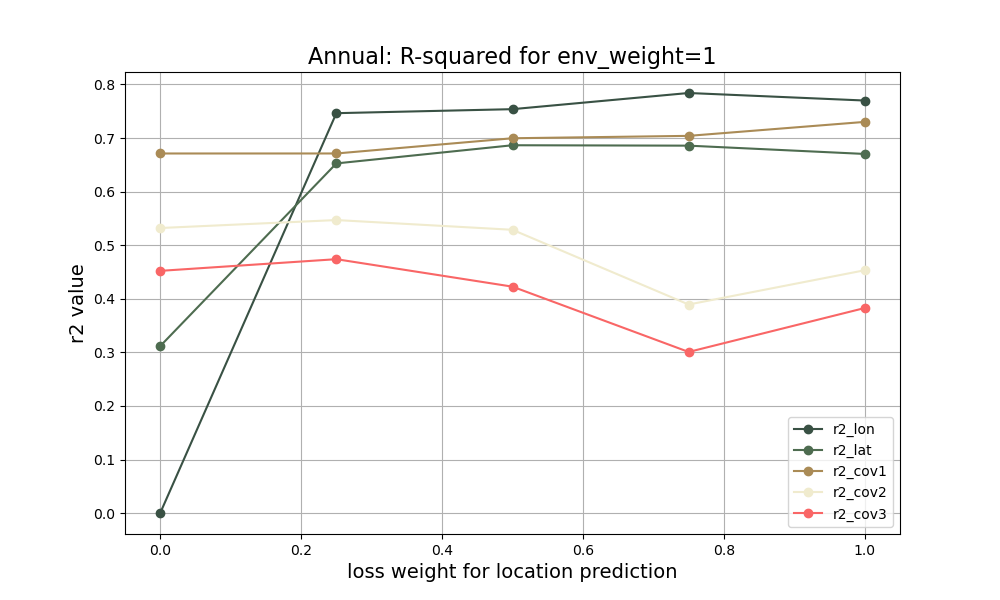
\includegraphics[width=\textwidth]{figures/suppfig1_lossweight_env.png}
        \caption{}
        \label{fig:S1a}
    \end{subfigure}
    \hfill
    \begin{subfigure}[t]{0.49\textwidth}
        \centering
        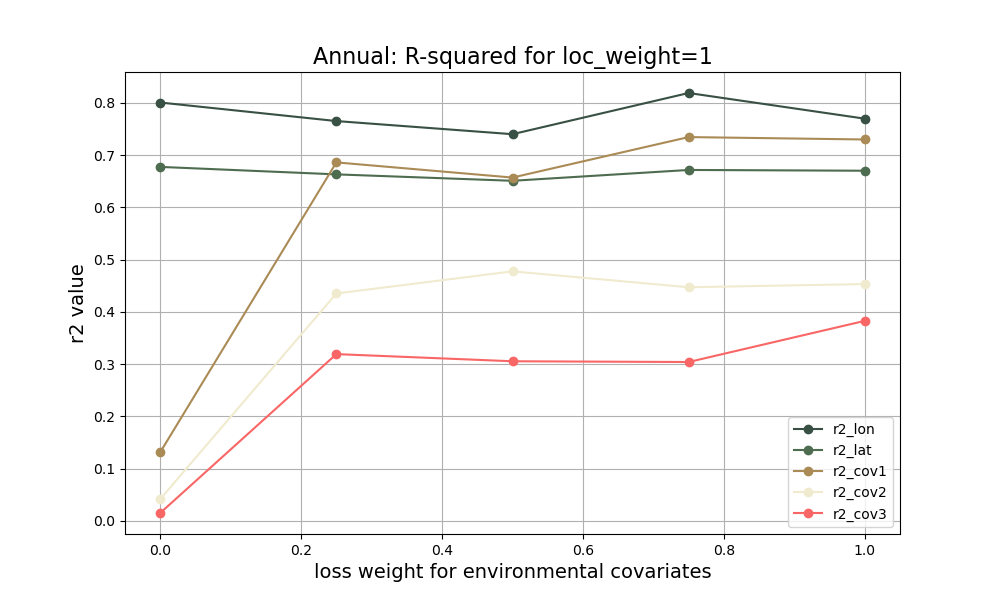
\includegraphics[width=\textwidth]{figures/suppfig1_lossweight_loc.png}
        \caption{}
        \label{fig:S1b}
    \end{subfigure}
    \caption{\textbf{Loss weight cross validation.}
    To determine the default loss weight value for location and
    environmental prediction, we tested sliding this value at the command
    line for each output task (location prediction and environmental
    covariate prediction) on the empirical \dfir{} data, while holding
    the other value at 1. In panel \textbf{a)}, we see that when the loss weight is
    held at a value of 0 for environmental covariate prediction, \ecolocator
    essentially ``focuses'' entirely on the location prediction task,
    reflected in the low R\textsuperscript{2} scores for all three environmental targets and
    high prediction scores for location. We see the same effect in the
    opposite direction in panel \textbf{b)}, where we held the loss weight of the
    environmental output head at 1 and scaled the loss weight for location
    prediction from 0--1. Again we see that when loss weight for location
    prediction is held at 0, the model prioritizes predicting on
    environmental covariates. Reassuringly, this analysis also demonstrates
    that \ecolocator recovers the true values for environmental covariates
    without over-reliance on the spatial information housed in the location
    values. Lastly, we see negligible effects of prediction performance in
    one output or the other when one output head is essentially turned
    off/down. Because of this, we hold the default value for both prediction
    tasks at 1.0.}
    \label{fig:S1}
\end{figure}

%%%%%% Supplemental Figure 2 %%%%%%
\begin{figure}[H]
    \centering
    \begin{subfigure}[t]{0.49\textwidth}
        \centering
        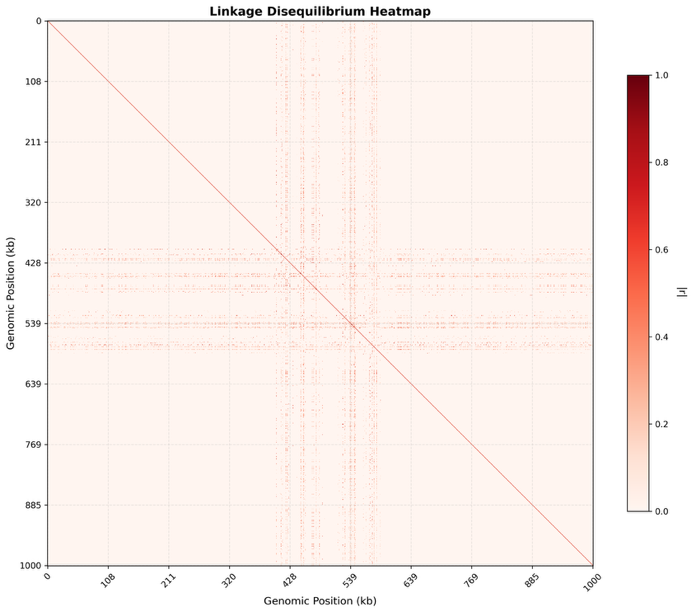
\includegraphics[width=\textwidth]{figures/suppfig2_LD_lowrecomb.png}
        \caption{}
        \label{fig:S2a}
    \end{subfigure}
    \hfill
    \begin{subfigure}[t]{0.49\textwidth}
        \centering
        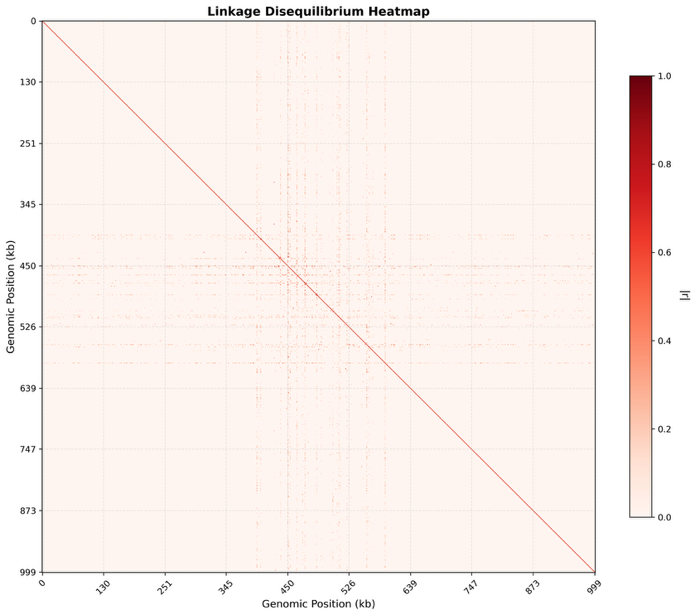
\includegraphics[width=\textwidth]{figures/suppfig2_LD_highrecomb.png}
        \caption{}
        \label{fig:S2b}
    \end{subfigure}
    \caption{\textbf{Linkage disequilibrium under different
    recombination rates for genomic architecture 1
    (\textbf{a)} Recombination = 10\textsuperscript{-8};
    \textbf{b)} Recombination = 10\textsuperscript{-6}).}
    Linkage disequilibrium between selected QTL windows and SNPs outside the
    selected region. To identify SNPs in linkage disequilibrium (LD) with
    the selected QTL window used in genetic architecture 1, we calculated
    pairwise correlations between SNPs inside the selected window and SNPs
    outside the window. These plots do not represent genome-wide LD decay or
    complete LD structure across the simulated genomic element; rather, they
    show the subset of outside-window SNPs that pass the LD threshold with
    SNPs in the selected region. Panel \textbf{a} shows LD partners under lower
    recombination, where LD extends more broadly away from the selected
    window. Under this parameterization, 525 SNP pairs showed very strong LD
    ($r^2 \geq 0.8$), 1,026 showed strong LD ($r^2 \geq 0.5$), and 2,923 showed moderate
    LD ($r^2 \geq 0.2$). Panel \textbf{b} shows the same analysis under higher
    recombination, where LD with the selected window is reduced. Under this
    parameterization, 9 SNP pairs showed very strong LD ($r^2 \geq 0.8$), 24
    showed strong LD ($r^2 \geq 0.5$), and 309 showed moderate LD ($r^2 \geq 0.2$).
    Because SNPs were filtered to include only LD partners of the selected
    QTL window, long-range LD in these panels should be interpreted as
    evidence of SNPs that remain correlated with the selected region, rather
    than as a general description of background LD across the genome.}
    \label{fig:S2}
\end{figure}

%%%%%% Supplemental Figure 3 %%%%%%
\begin{figure}[H]
    \centering
    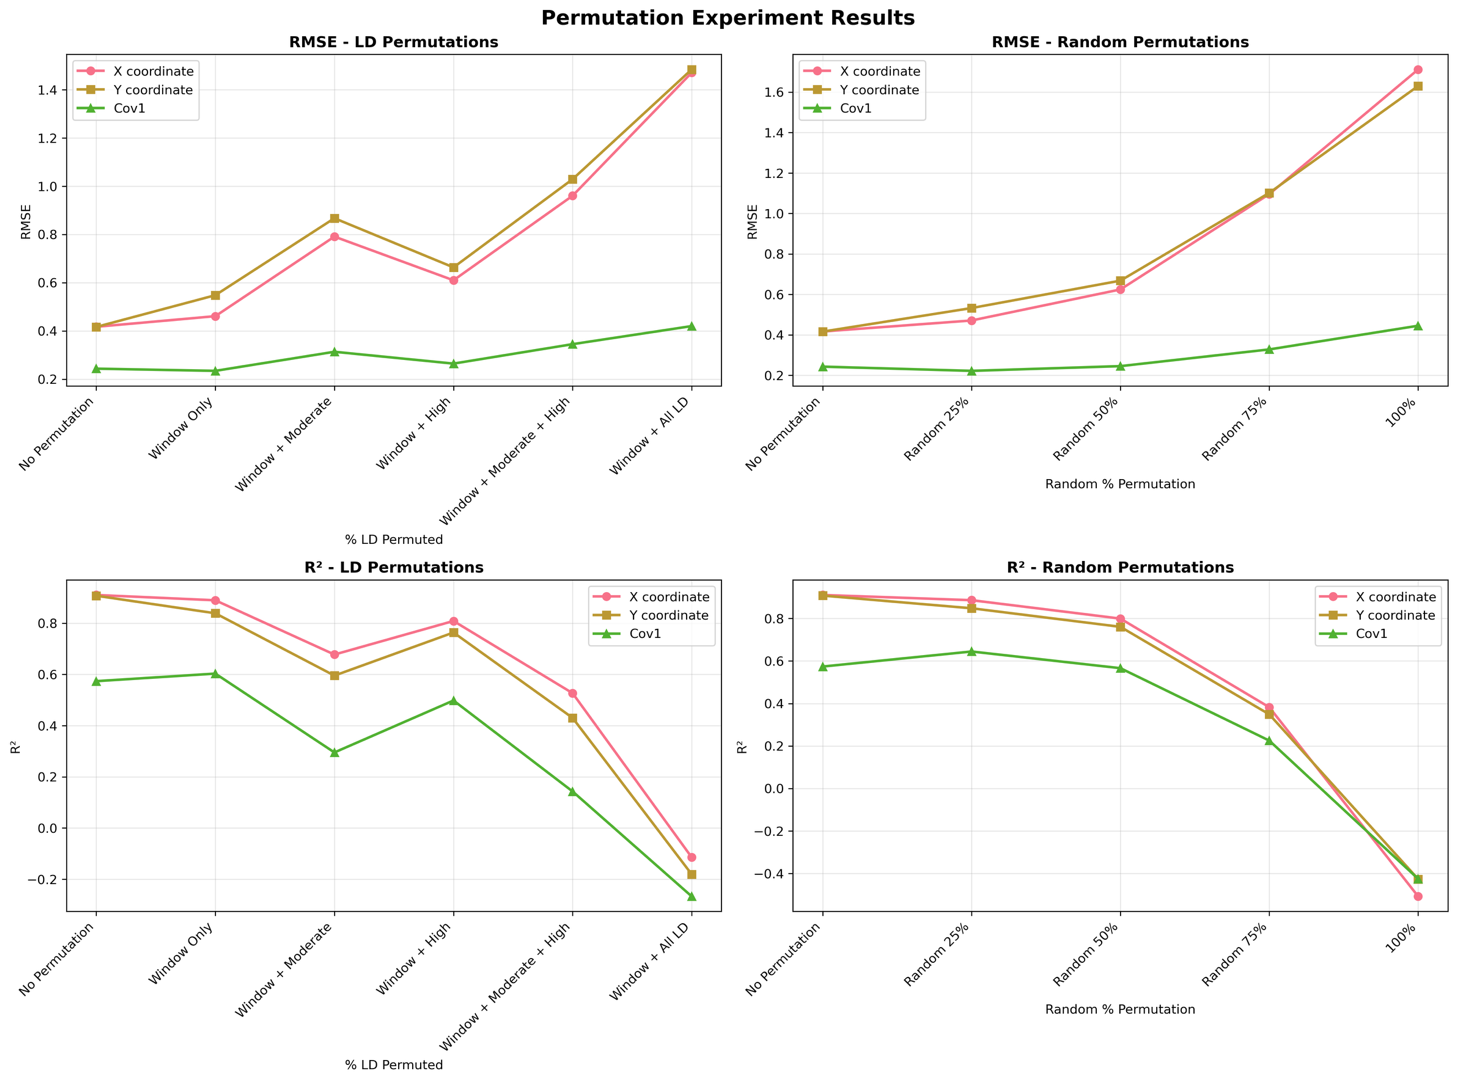
\includegraphics[width=\textwidth]{figures/suppfig3_permutation.png}
    \caption{\textbf{RMSE and R\textsuperscript{2} of \ecolocator predictions under
    different permutation regimes (combinations of random \% permuted and
    sites in LD permuted).}
    \ecolocator prediction performance under random and LD-targeted
    permutation regimes. To assess whether prediction accuracy depends
    primarily on the selected QTL window, SNPs in linkage disequilibrium
    with that window, or genome-wide signal distributed across the genotype
    matrix, we permuted subsets of the genotype matrix across individuals
    prior to prediction. The left column shows targeted permutations of the
    selected window alone and the selected window combined with SNPs in
    moderate, high, or all LD with the selected region. The right column
    shows random genome-wide permutations of increasing proportions of SNPs.
    The top row shows root mean squared error (RMSE), and the bottom row
    shows R\textsuperscript{2} for X coordinate (longitude), Y coordinate (latitude), and the
    environmental covariate. In both permutation designs, prediction
    accuracy declines as more genotype information is shuffled, indicating
    that \ecolocator relies on genetic signal distributed across the genotype
    matrix. However, permuting the selected window together with all
    LD-linked sites causes a sharp loss of performance, suggesting that SNPs
    correlated with the selected region carry important predictive
    information. Randomly permuting all SNPs produces similarly poor
    performance, confirming that prediction accuracy is lost when
    genotype--environment and genotype--location associations are fully
    disrupted. Note that the ``window + all LD'' grouping comprised roughly
    75\% of sites, so comparing that to the random 75\% permutation again
    reiterates the importance of SNPs in LD.}
    \label{fig:S3}
\end{figure}

%%%%%% Supplemental Figure 4 %%%%%%
\begin{figure}[H]
    \centering
    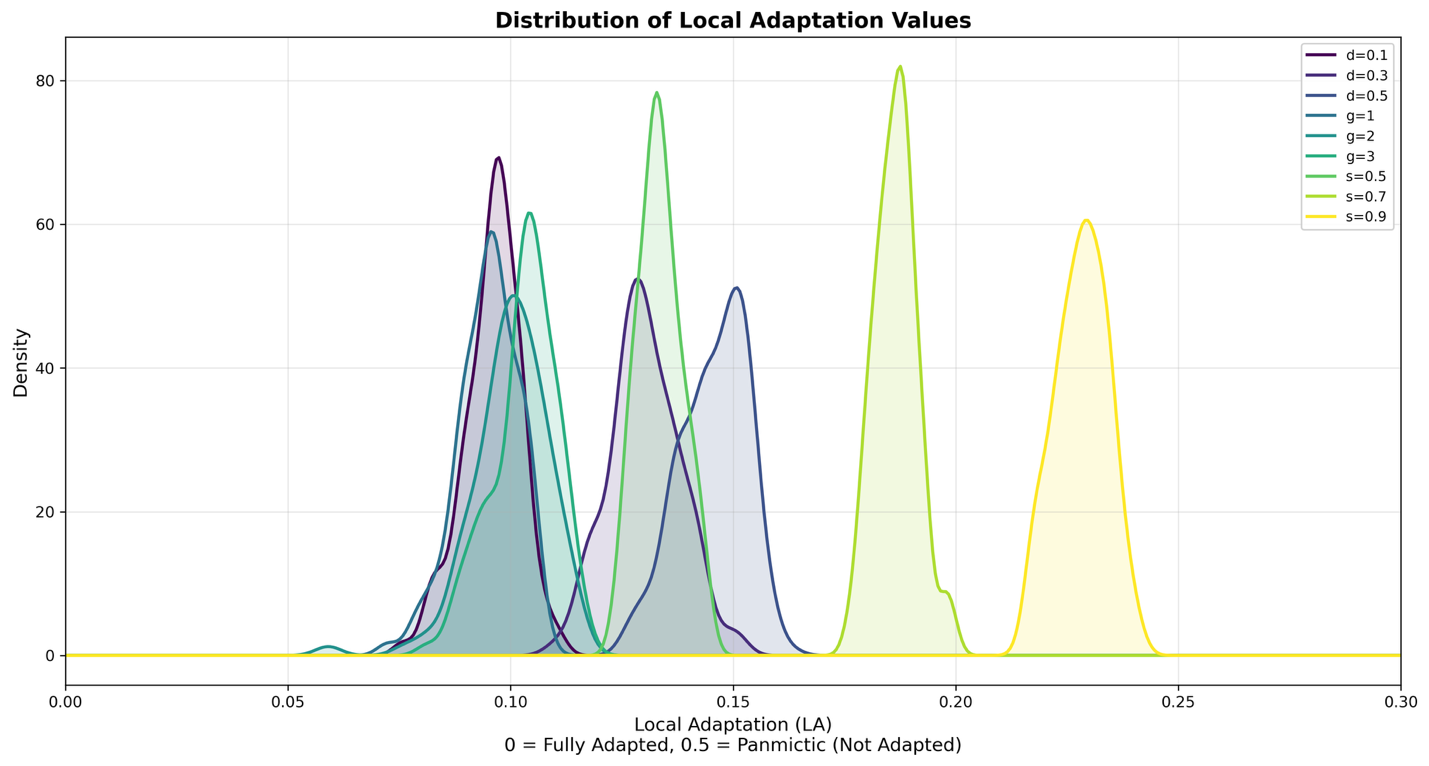
\includegraphics[width=\textwidth]{figures/suppfig4_localadaptation.png}
    \caption{\textbf{Distribution of strength of local adaptation across parameter space.}
    Kernel density estimates of local adaptation (LA) values for 100
    simulation replicates per parameter combination across three parameter
    explorations on an 8\texttimes 8 grid-like landscape with Hurst = 0 (no
    autocorrelation between space and environment). LA is calculated as the
    mean absolute difference between individual phenotypic values and their
    local optima; lower values indicate stronger local adaptation. The
    selection parameter $s$ controls the standard deviation of the fitness
    function, where smaller values produce a tighter fitness distribution
    and thus stronger selection. Dispersal ($d$ = 0.1, 0.3, 0.5; genetic
    architecture 1 and $s$ = 0.5 fixed): increasing dispersal progressively
    eroded local adaptation, with mean LA values of 0.096, 0.130, and 0.146
    for $d$ = 0.1, 0.3, and 0.5, respectively. Genetic architecture ($g$ = 1, 2,
    3; $d$ = 0.1 and $s$ = 0.5 fixed): distributing QTLs increasingly across the
    genomic element had a modest effect on local adaptation, with mean LA
    values of 0.095, 0.100, and 0.103 for $g$ = 1, 2, and 3, respectively.
    Selection ($s$ = 0.5, 0.7, 0.9; genetic architecture 1 and $d$ = 0.3 fixed):
    weaker selection substantially reduced local adaptation, with mean LA
    values of 0.134, 0.187, and 0.228 for $s$ = 0.5, 0.7, and 0.9,
    respectively.}
    \label{fig:S4}
\end{figure}

%%%%%% Supplemental Figure 5 %%%%%%
\begin{figure}[H]
    \centering
    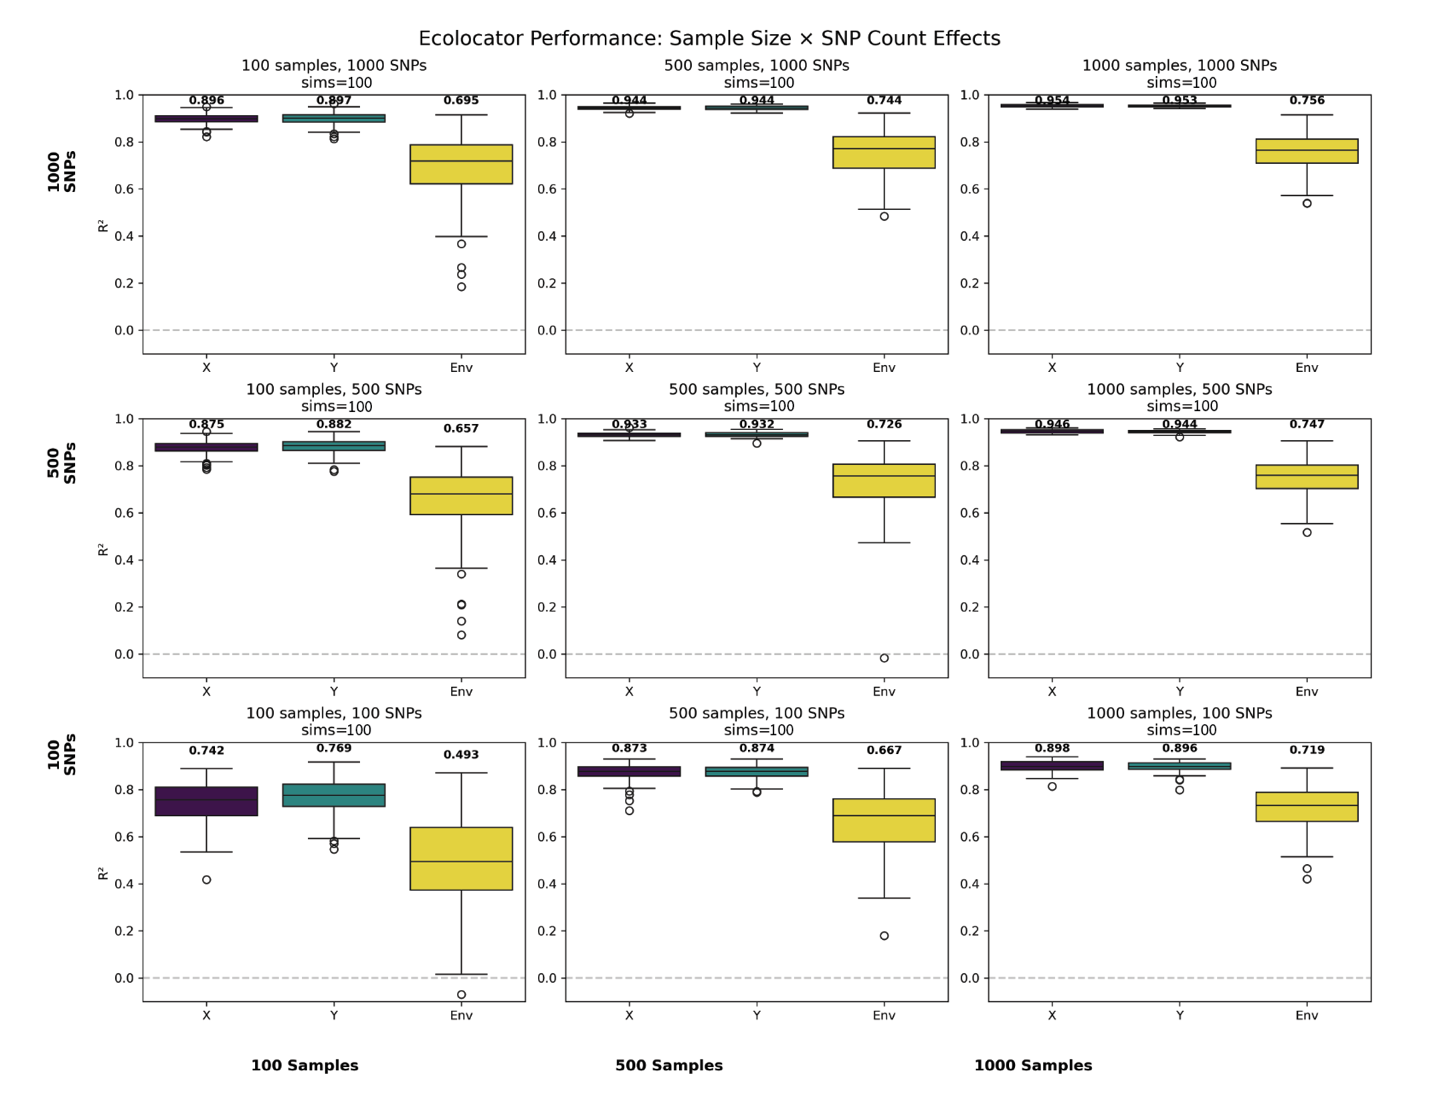
\includegraphics[width=\textwidth]{figures/suppfig5_downsampling.png}
    \caption{\textbf{Effects of down-sampling individuals and SNPs as input to \ecolocator.}
    \ecolocator performance under various downsampling regimes of the same
    simulated data ($d$ = 0.1, $s$ = 0.5, $g$ = 1). In the top row, there are 1000 SNPs
    made available to the model; in the middle and bottom rows, there are
    500 and 100 SNPs respectively. In the columns we vary sample size, with
    100, 500, and 1000 samples from left to right. R\textsuperscript{2} values across 100
    simulation replicates are summarized in boxplots, with Longitude (x) in
    purple, Latitude (y) in teal, and Environment in yellow. Because
    \ecolocator learns from variation present in the data, it is no surprise
    that we observe the highest prediction accuracy across targets
    (Lon. R\textsuperscript{2} = 0.954, Lat. R\textsuperscript{2} = 0.953, and Env. R\textsuperscript{2} = 0.756) with 1000 samples and
    1000 SNPs (top right corner), and we see the lowest prediction accuracy
    (Lon. R\textsuperscript{2} = 0.742, Lat. R\textsuperscript{2} = 0.769, and Env. R\textsuperscript{2} = 0.493) with only 100
    SNPs and 100 samples (bottom left corner). Under the sample sizes and
    SNP sets explored here, we do not observe diminishing returns with ``too
    much'' data being shown to the model, and similarly, we do not see a
    complete absence of predictive performance when sample size and SNP set
    are restricted.}
    \label{fig:S5}
\end{figure}

%%%%%% Supplemental Figure 6 %%%%%%
\begin{figure}[H]
    \centering
    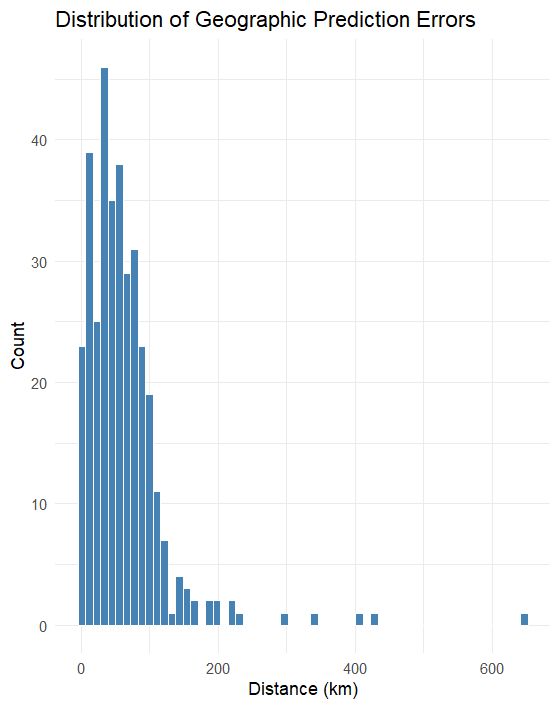
\includegraphics[width=0.5\textwidth]{figures/suppfig6_geoerror.png}
    \caption{\textbf{Distribution of geographic prediction errors on \dfir{} data.}
    A histogram of geographic distance prediction errors in our
    empirical application of Ecolocator on the \dfir case study data.
    Distance in kilometers (km) is on the x-axis and count is on the y-axis. 
    Most errors fall between 0-100km, with others as high as $>$600km.}
    \label{fig:S6}
\end{figure}

%%%%%% Supplemental Figure 7 %%%%%%
\begin{figure}[H]
    \centering
    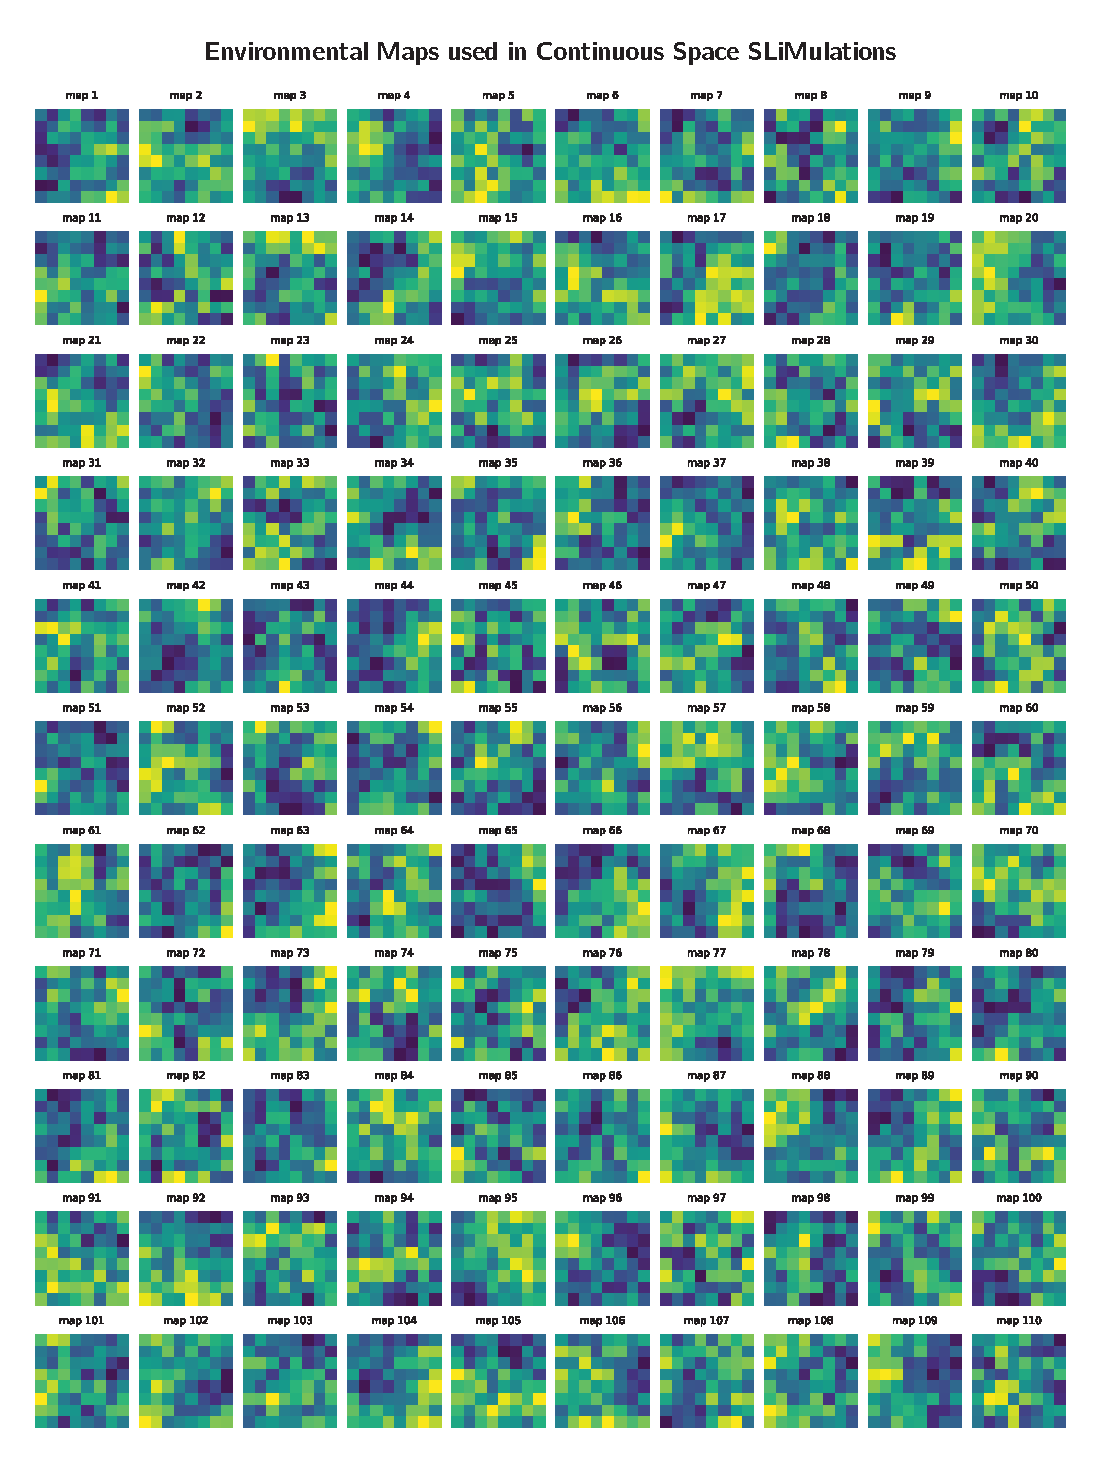
\includegraphics[width=\textwidth]{figures/suppfig7_envmaps.pdf}
    \caption{\textbf{Environmental Maps used in Continuous Space SLiMulations.}
    Environmental maps generated with the \texttt{NLMpy} python package 
    with pixel count set to 8x8 and hurst (autocorrelation)
    set to H=0. We generated 110 maps and sampled 100 of them randomly
    for each simulation regime we simulated. }
    \label{fig:S7}
\end{figure}

%%%%%% Supplemental Figure 8 %%%%%%
\begin{figure}[H]
    \centering
    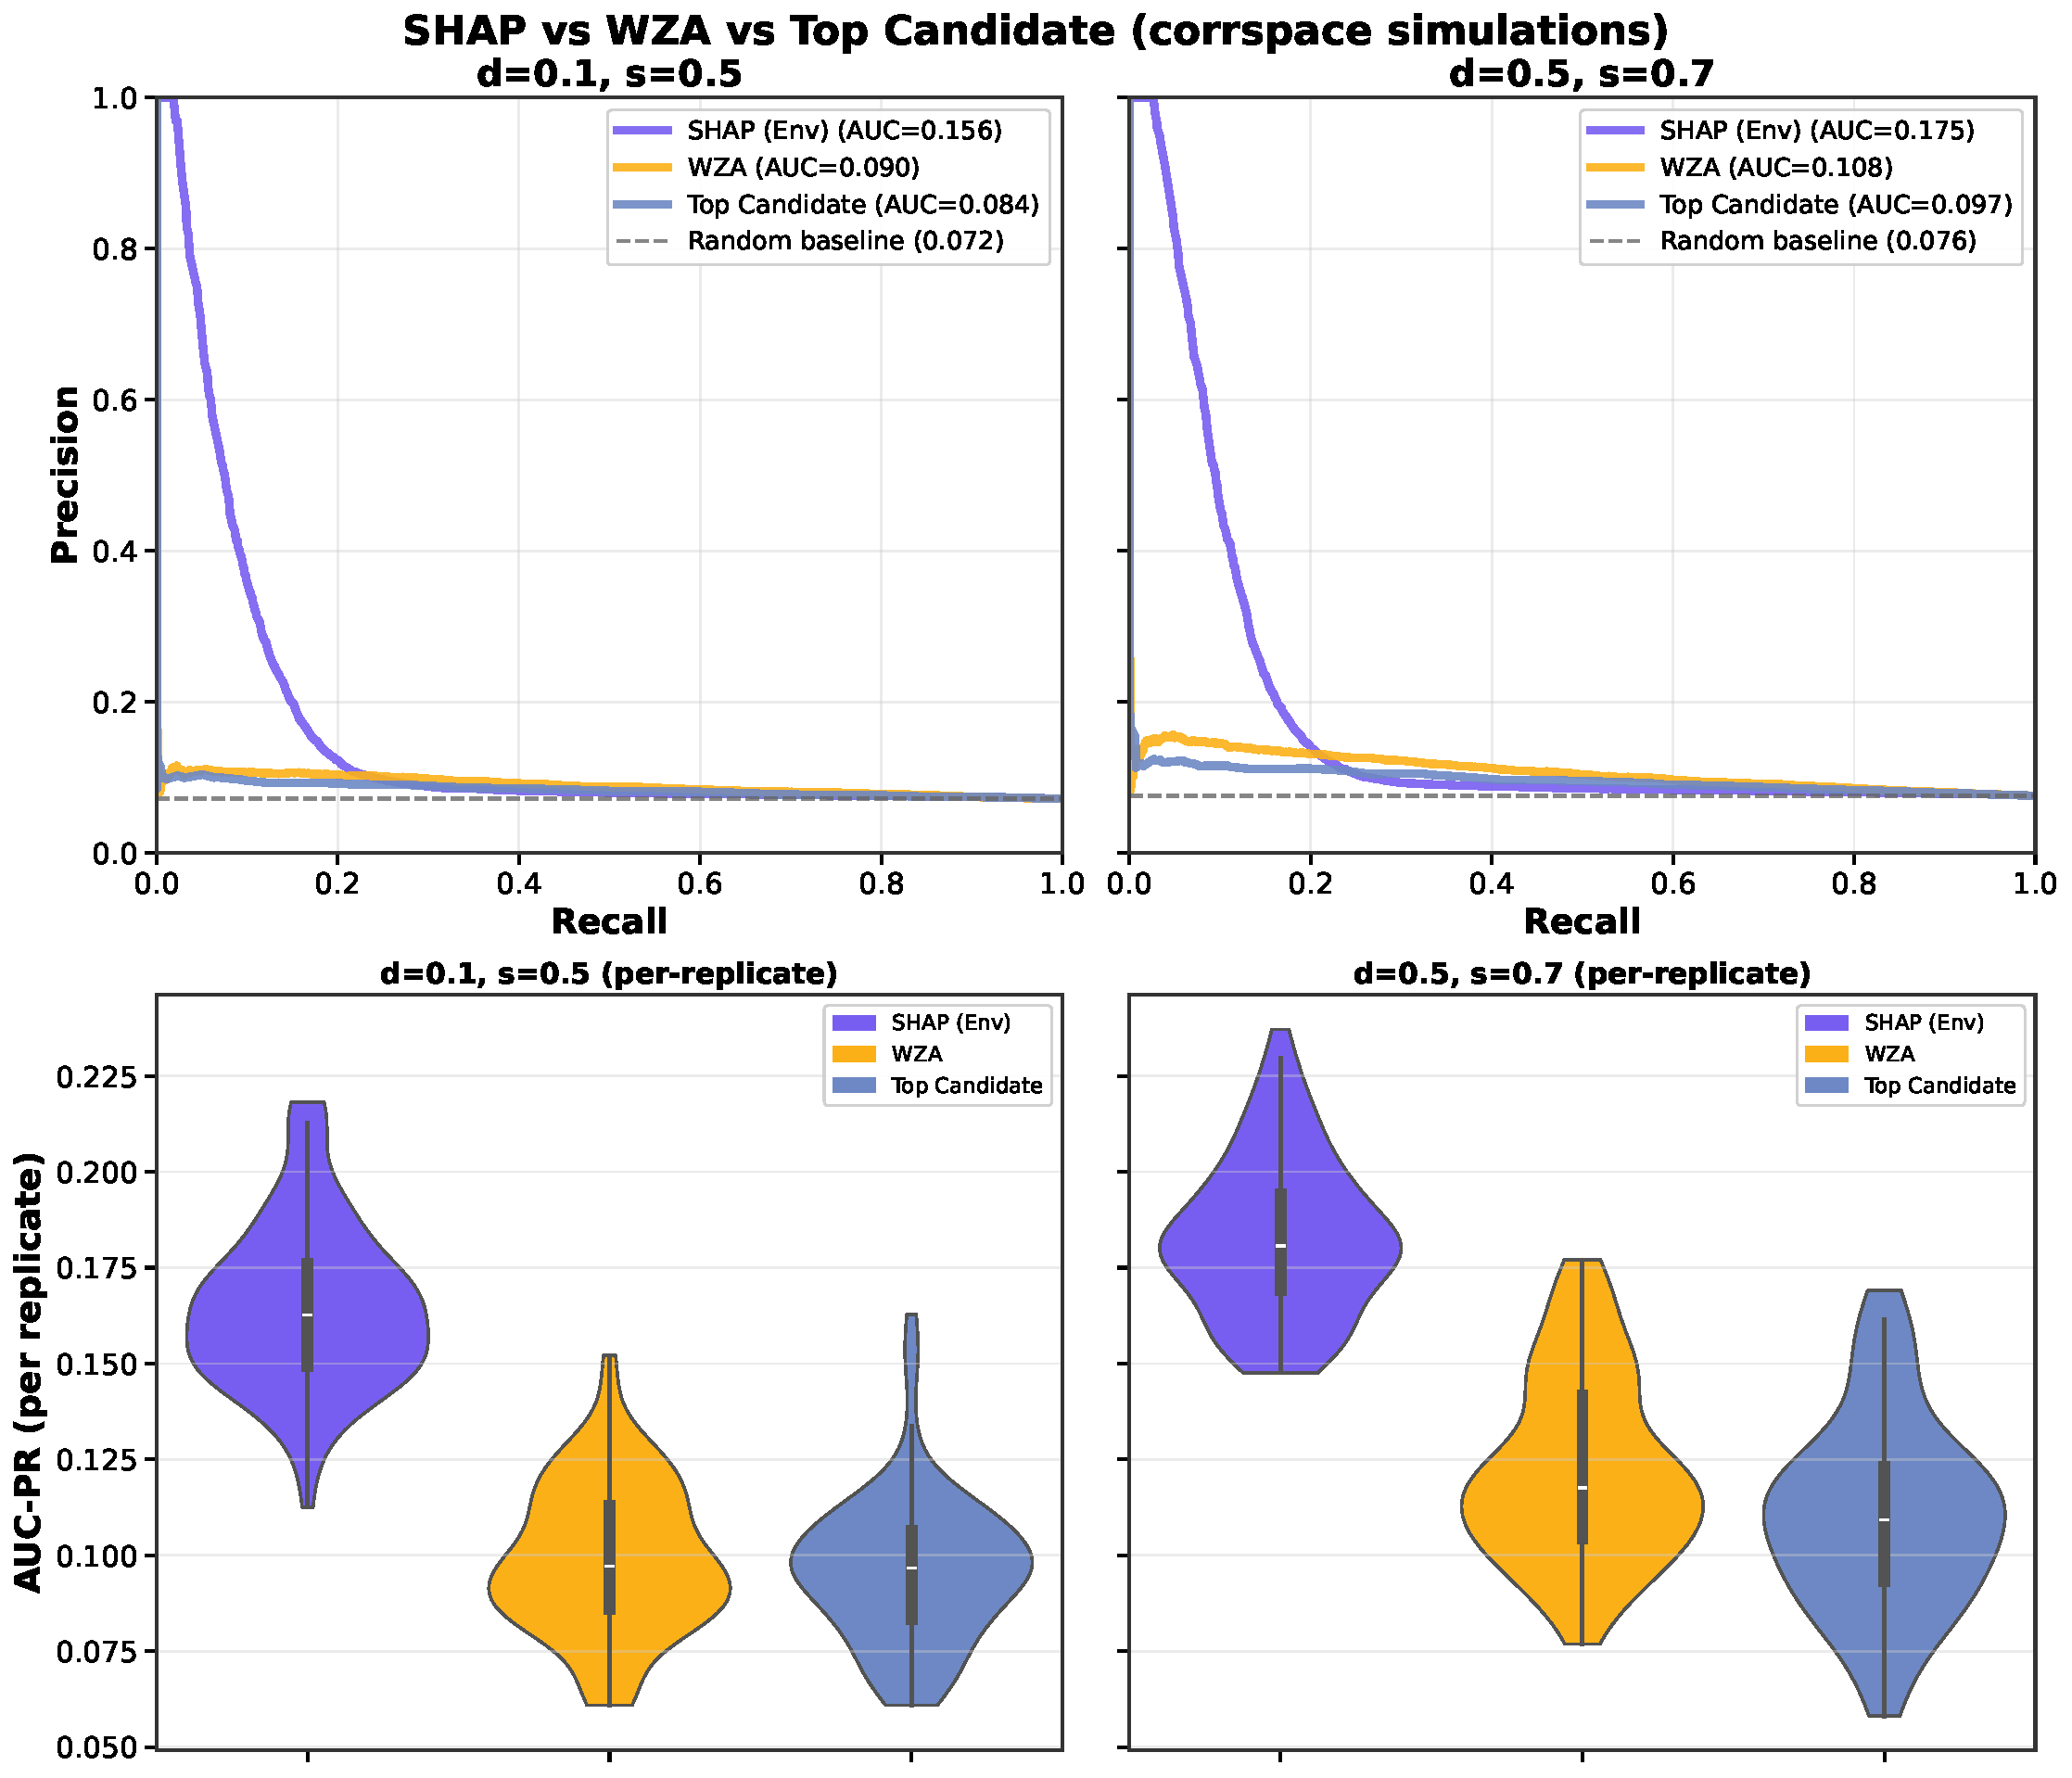
\includegraphics[width=\textwidth]{figures/suppfig8_shap_wza_topcan_aucpr_corrspace.pdf}
    \caption{\textbf{AUC-PR of Ecolocator/SHAP, WZA, and Top-Candidate GEA Methods Across Two Dispersal/Selection Regimes.}
    Precision-recall curves (top) and per-replicate AUC-PR violin plots (bottom) comparing three
    genotype-environment association methods for identifying adaptive SNPs: Ecolocator/SHAP (purple;
    mean $\lvert\mathrm{SHAP}\rvert$ for the environmental covariate, ranked by an empirical false-discovery-proportion 
    score computed from known ground-truth adaptive status), WZA (yellow), and top-candidate (blue). 
    Top row: precision-recall curves pooling all SNPs across 100 simulation replicates per regime, 
    scored by $-\log_{10}$(p-value) against true adaptive status;
    dashed line = random-baseline AUC-PR (proportion of adaptive SNPs). Bottom row: distribution of
    AUC-PR computed separately within each of the 100 replicates, showing the consistency of each
    method's performance across independent simulations. Left: limited-dispersal, strong-selection
    regime (dispersal=0.1, std.\ dev.\ of fitness function=0.5). Right: higher-dispersal, weaker-selection
    regime (dispersal=0.5, std.\ dev.\ of fitness function=0.7). Ecolocator/SHAP outperforms WZA and
    top-candidate under both regimes, both pooled and at the per-replicate level.}
    \label{fig:S8}
\end{figure}

%%%%%% Supplemental Figure 9 %%%%%%
\begin{figure}[H]
    \centering
    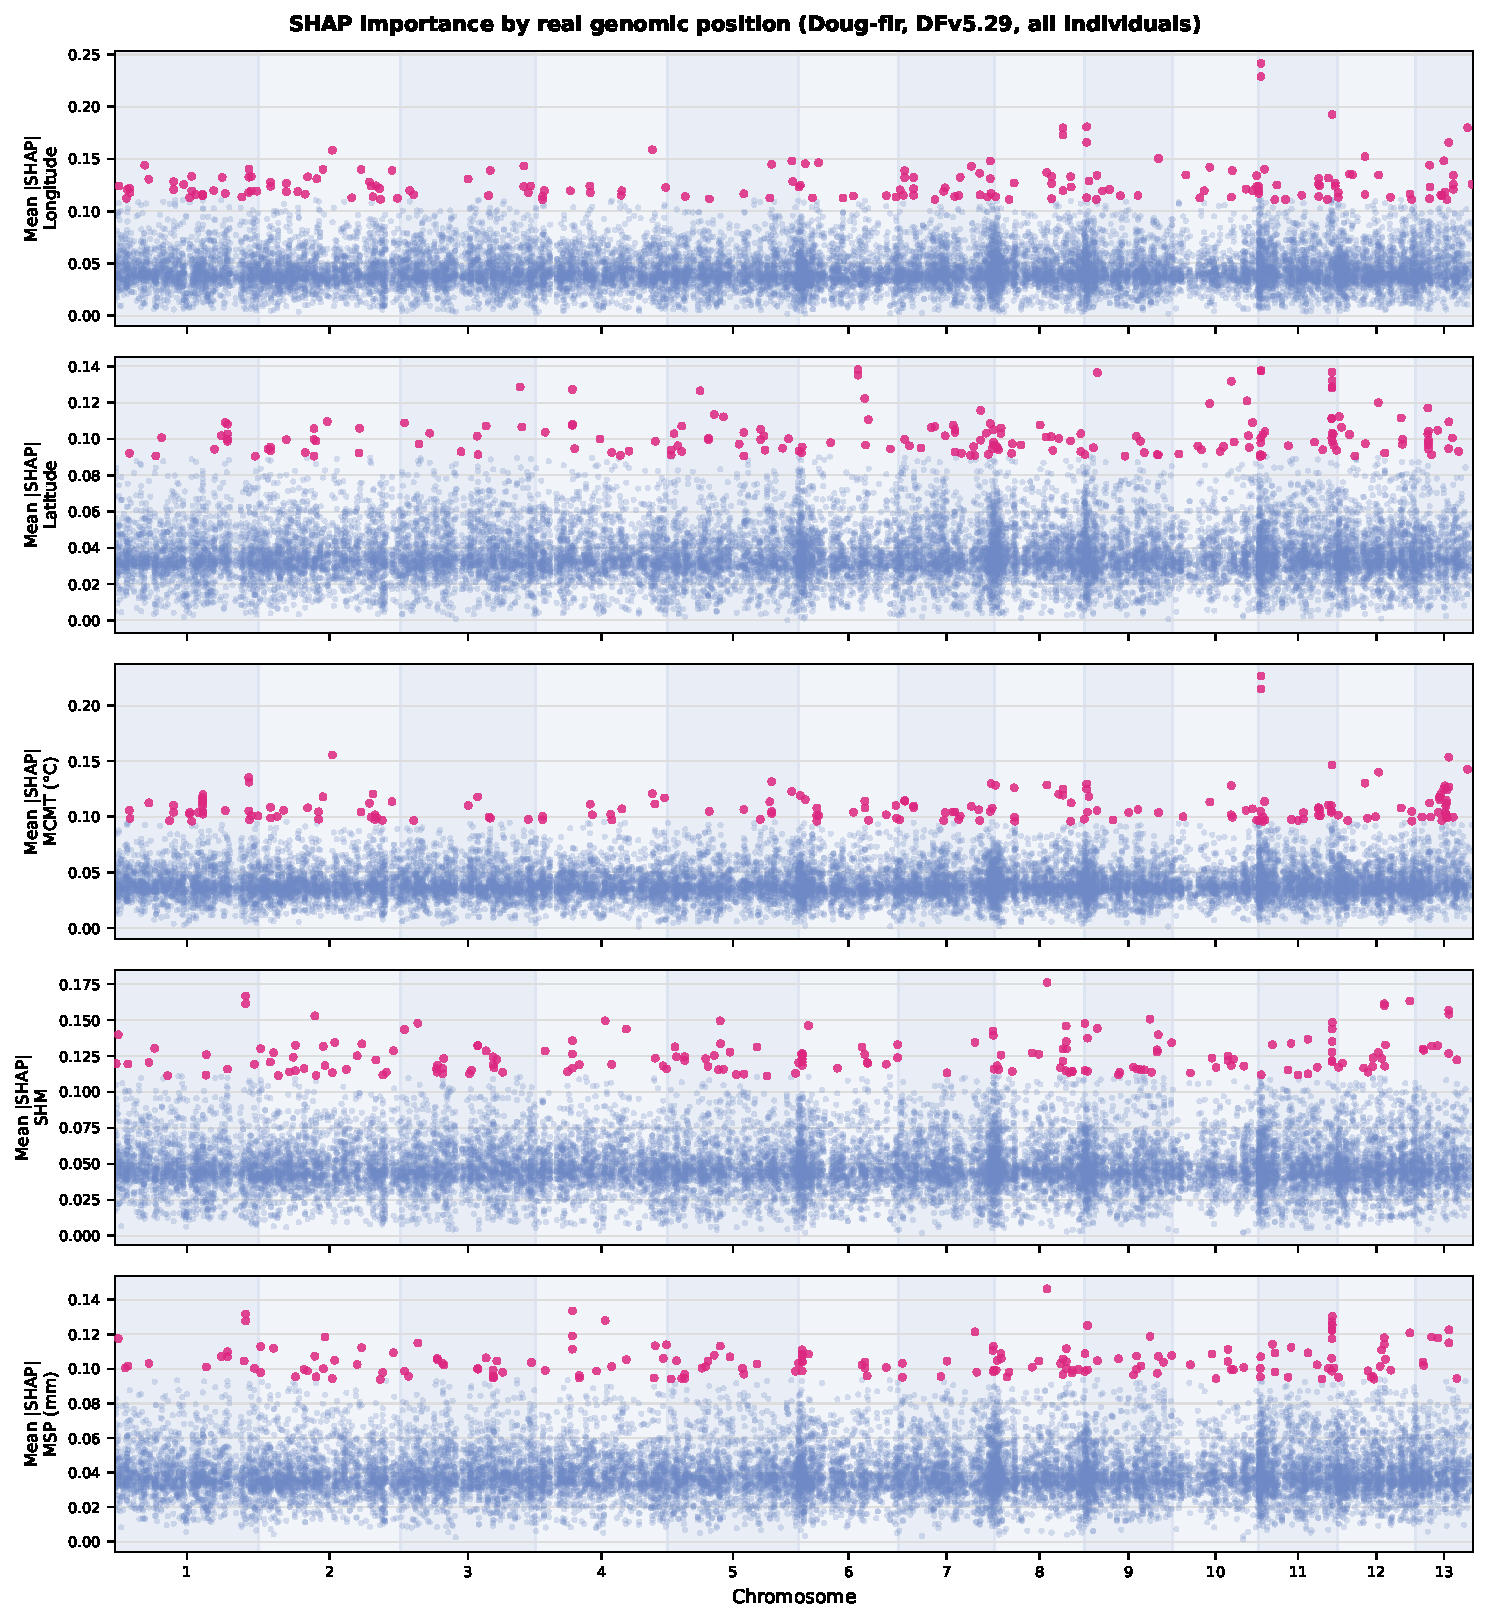
\includegraphics[width=\textwidth]{figures/suppfig9_shap_manhattan_dfir_positional.pdf}
    \caption{\textbf{Mean $\lvert\mathrm{SHAP}\rvert$ by Real Genomic Position Across Five Prediction Targets for Douglas-fir.}
    Manhattan-style plots of mean $\lvert\mathrm{SHAP}\rvert$ (averaged across leave-one-out
    cross-validation folds) at real chromosomal positions (chromosomes 1--13, Douglas-fir reference
    assembly DFv5.29; SNP positions resolved by SAM alignment restricted to primary, high-confidence
    mappings, MAPQ $\geq$ 30) for five prediction targets, top to bottom: longitude, latitude, mean
    coldest-month temperature (MCMT), summer heat:moisture index (SHM), and mean summer precipitation
    (MSP). SNPs in the top 1\% of mean $\lvert\mathrm{SHAP}\rvert$ for a given target are highlighted
    in pink; all other SNPs are shown in blue. Alternating background shading demarcates chromosome
    boundaries.}
    \label{fig:S9}
\end{figure}

%%%%%% Supplemental Figure 10 %%%%%%
\begin{figure}[H]
    \centering
    
\includegraphics[width=\textwidth]{figures/suppfig10_LA_greyscale4.png}
    \caption{\textbf{Environmental Map used in Correlated Space Simulations.}
    A greyscale left-right gradient image used in simulations to represent 
    an arbitrary environmental variable correlated with space along the longitudinal axis.}
    \label{fig:S10}
\end{figure}

%%%%%% Supplemental Figure 11 %%%%%%
\begin{figure}[H]
    \centering
    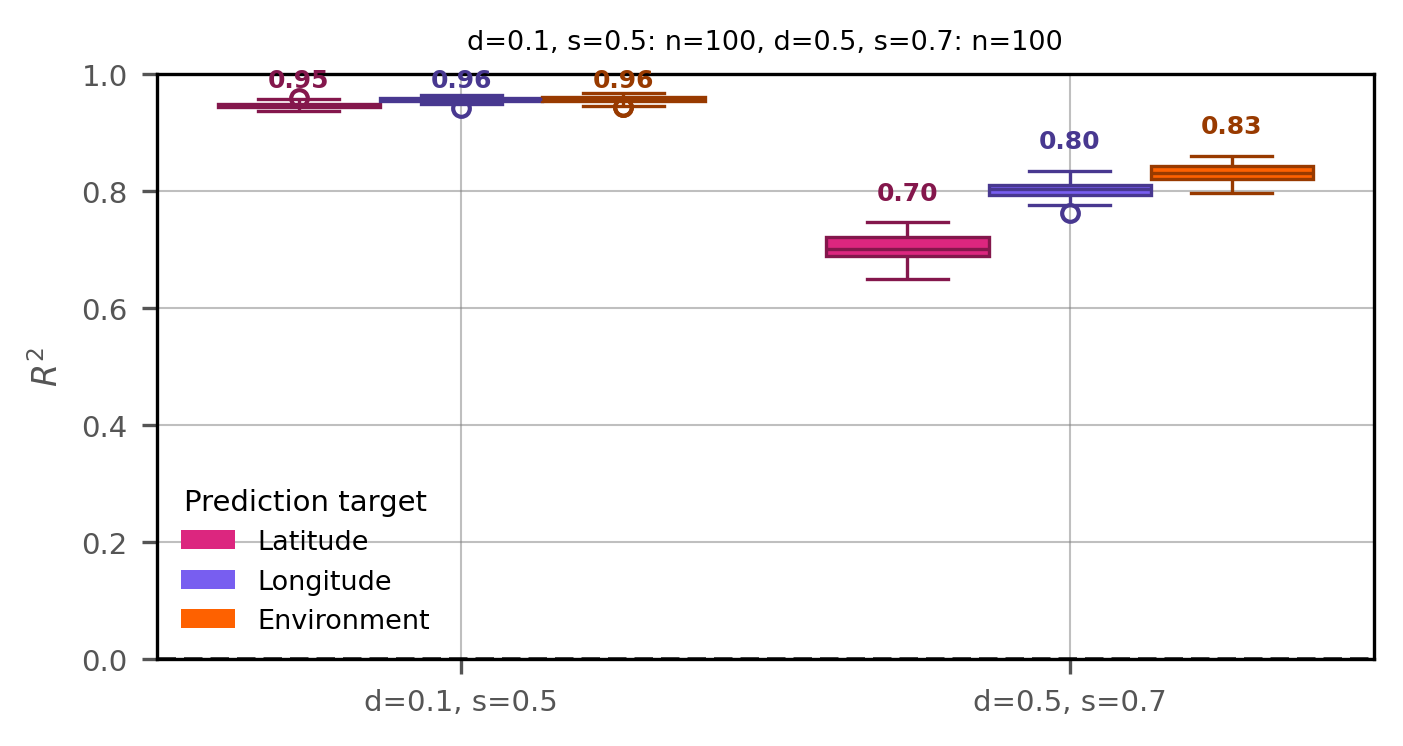
\includegraphics[width=\textwidth]{figures/suppfig11_loo_r2_boxplots_both_regimes.png}
    \caption{\textbf{Per-replicate LOOCV prediction accuracy (R²) across two dispersal/selection regimes.}
    For each of 100 independent simulation replicates per regime, 
    predictions from all leave-one-out cross-validation folds 
    were pooled and compared to the known sampled values to 
    compute a single R² per replicate for each of three prediction 
    targets: latitude, longitude, and environment (cov1). 
    Boxplots show the distribution of these per-replicate R² 
    values (box = interquartile range, line = median, whiskers = 1.5×IQR, 
    points beyond whiskers = outlier replicates); numbers above each box 
    give the across-replicate mean R². Left: limited-dispersal, 
    strong-selection regime (d=0.1, s=0.5). Right: higher-dispersal, 
    weaker-selection regime (d=0.5, s=0.7). Prediction accuracy 
    is uniformly high and tightly distributed for all three targets 
    under limited dispersal/strong selection (mean R²=0.95–0.96), 
    but declines and becomes more variable across replicates under higher 
    dispersal/weaker selection, most notably for latitude 
    (mean R²=0.70 vs. 0.80–0.83 for longitude and environment).}
    \label{fig:S11}
\end{figure}

%%%%%% Supplemental Figure 12 %%%%%%
\begin{figure}[p]
    \centering
    \adjustimage{width=1.3\textwidth, max totalheight=0.9\textheight, center}{figures/suppfig12_shap_manhattan_alltargets_rep1.pdf}
    \caption{\textbf{Genomic Distribution of Mean $\lvert\mathrm{SHAP}\rvert$ Across Three Prediction Targets in a Representative Replicate.}
    Mean $\lvert\mathrm{SHAP}\rvert$ by genomic position (bp) for one representative simulation
    replicate (rep1), shown for three prediction targets (rows: latitude, longitude, environment) and
    both dispersal/selection regimes (columns: limited-dispersal, strong-selection, dispersal=0.1,
    std.\ dev.\ of fitness function=0.5, left; higher-dispersal, weaker-selection, dispersal=0.5,
    std.\ dev.\ of fitness function=0.7, right). SNPs classified as non-neutral (true causal loci or in
    linkage disequilibrium with a causal locus; magenta, black-outlined) are overlaid on all other
    neutral/LD-linked SNPs (light blue).}
    \label{fig:S12}
\end{figure}
\clearpage

%%%%%% Supplemental Table 1 %%%%%%
\begin{table}[ht]
  \centering
  \caption{\textbf{R\textsuperscript{2} values for \ecolocator climate variable predictions versus ClimateNA modelled values from predicted locations.}}
  \label{tab:supptable1}
  \begin{tabular}{@{}p{6.5cm}cc@{}}
  \hline
  \textbf{Predicted Location and Climate} & \shortstack{\textbf{Geolocation and}\\ \textbf{Climate Prediction}} & \shortstack{\textbf{Geolocation}\\ \textbf{and ClimateNA}} \\
  \hline
  Latitude (LAT, \textdegree) & 0.84 & -- \\
  Longitude (LON, \textdegree) & 0.76 & -- \\
  Mean Cold Month Temperature (MCMT, \textdegree C) & 0.75 & 0.65 \\
  May to September Precipitation (MSP, mm) & 0.51 & 0.31 \\
  Summer heat:moisture index (SHM, \textdegree C/um) & 0.53 & 0.30 \\
  \hline
  \end{tabular}
\end{table}

%%%%%% Supplemental Table 2 %%%%%%
\begin{table}[ht]
  \centering
  \caption{\textbf{Mean R\textsuperscript{2} values for \ecolocator predictions of longitude, latitude, and environment across simulation types.}}
  \label{tab:supptable2}
  \begin{tabular}{@{}llccc@{}}
  \hline
  \textbf{Simulation type} & \textbf{Parameter} & \textbf{Longitude R\textsuperscript{2}} & \textbf{Latitude R\textsuperscript{2}} & \textbf{Environment R\textsuperscript{2}} \\
  \hline
  Wright-Fisher (discrete space) & -- & 0.986 & 0.985 & 0.916 \\
  \hline
  \multirow{9}{*}{Non-Wright-Fisher (continuous space)}
   & $g=1$ & 0.967 & 0.967 & 0.759 \\
   & $g=2$ & 0.967 & 0.967 & 0.771 \\
   & $g=3$ & 0.968 & 0.968 & 0.787 \\
   \cline{2-5}
   & $s=0.3$ & 0.917 & 0.916 & 0.609 \\
   & $s=0.5$ & 0.911 & 0.911 & 0.561 \\
   & $s=0.7$ & 0.906 & 0.907 & 0.421 \\
   \cline{2-5}
   & $d=0.1$ & 0.968 & 0.967 & 0.769 \\
   & $d=0.3$ & 0.912 & 0.911 & 0.556 \\
   & $d=0.5$ & 0.815 & 0.814 & 0.336 \\
  \hline
  \end{tabular}
\end{table}




\end{document}
